\documentclass[11pt]{article}

% ---------------------------------------------------------------- preamble
\usepackage[margin=1in]{geometry}
\usepackage{amsmath,amssymb,amsthm}
\usepackage{graphicx}
\usepackage{booktabs}
\usepackage{algorithm}
\usepackage{algorithmic}
\usepackage{microtype}
\usepackage{xcolor}
\usepackage{tikz}
\usetikzlibrary{arrows.meta,positioning,patterns,calc}
\usepackage[font=small,labelfont=bf]{caption}
\usepackage{natbib}
\newcommand{\kwta}{$k$-WTA}
\usepackage[colorlinks=true,linkcolor=blue!60!black,citecolor=blue!60!black,urlcolor=blue!60!black]{hyperref}

\newtheorem{proposition}{Proposition}
\newtheorem{corollary}{Corollary}
\newtheorem{definition}{Definition}
\newtheorem{remark}{Remark}

% Placeholder for results still being produced (phase 11 runs in progress).
\newcommand{\pending}[1]{\textcolor{orange!80!black}{\textbf{[PENDING:} #1\textbf{]}}}

\title{Inference as Consolidation: Replay in the Silent Degrees of Freedom}

\author{%
  Anonymous author(s)\\[2pt]
  \small Affiliation withheld for double-blind review}
\date{Preprint, draft of \today}

\begin{document}
\maketitle

% ---------------------------------------------------------------- abstract
\begin{abstract}
Biological brains consolidate memories both in dedicated offline states (sleep) and, as recent
causal evidence shows, through \emph{local sleep}: brief, use-dependent off-periods of individual
cortical circuits during wakefulness. In contrast, replay-based continual learning in artificial
neural networks almost universally relies on offline consolidation phases or on interleaving
replayed samples with the input stream. We ask whether a network trained end-to-end by local,
biologically constrained learning rules can consolidate \emph{during inference}, with no offline
phase at all. We introduce (i) a \emph{refractory rotation} rule under which units that have just
fired sit out the next competition, (ii) an \emph{isolation} scheme that confines replay
updates to hidden synapses invisible to the current input under $k$-winner-take-all (\kwta)
dynamics --- exact for silent presynaptic and suppressed units, and measured to alter the
waking hidden code of only $0.2$--$0.4\%$ of samples per replay step elsewhere --- with
per-synapse optimiser state advanced only inside the mask, and (iii) internal control signals
--- a unit-level homeostatic pressure that triggers replay bursts, and a relative-novelty
(fast-over-slow error) gate that decides when rotation runs. The construction inverts the usual
direction of non-interfering continual learning: rather than protecting past tasks while learning
the present one, the hidden computation on the current input, under its suppression mask, is
held invariant --- exactly on the proven channels, and for all but $0.3\%$ of waking hidden
codes per update elsewhere --- while past memories are consolidated
through degrees of freedom the current batch exposes as unused. On class-incremental split-MNIST the
resulting system reaches $\mathbf{91.6\pm0.3\%}$ (six seeds) with no offline phase, exceeding
the best offline-night schedule ($89.2\pm1.7\%$) at $2.4\times$ the night's replay samples
(and reaching $91.1\pm0.4\%$ within $1.2\times$ of that budget with eight-sample
micro-batches); reversing the protected direction (guarding past memories
while learning the present, as in null-space methods) costs fourteen points under identical machinery; rotation carries the gain (rotation with
unmasked replay reaches $91.5\pm0.3\%$; isolation adds $0.1$--$0.3$ points at replay batches of
$16$ to $4$, the guarantee, and at two-sample batches the absence of the collapse that unmasked
replay shows in half the seeds; $2.6$ points without rotation); every reported number is measured on
held-out training data never used for any decision, and the headline orderings hold on a
second, independent split. Rotation's i.i.d.\ price is governed by the substrate's activity fraction: at the $5\%$
fraction used in the earlier phases of this work, novelty gates (masked Adam) or
sleep-bout-committed gates (heavy-ball SGD) were needed to refund it, whereas at the $10\%$
optimum the price shrinks to one to two points and both gates become neutral --- increasing the
activity fraction reduced the price more consistently than any tested gate.
On split CIFAR-10 the ordering of methods transfers and widens, and a substrate decomposition
shows that the remaining gap to backpropagation-with-replay is dense activation, not credit
assignment. Finally, a drive-referenced controller for the rule's synaptic decay --- one
dataset-independent ratio target in place of per-dataset tuning --- trades $1$--$3$ sequential points for static gains on every CIFAR regime and lifts the system
onto 100-class streams
that defeat the tuned fixed decay without skips; with locally learned ResNet-style skip
synapses the five-hidden-layer stack then holds the two-hidden-layer level on both axes. We provide
exactness
proofs for the isolation rule and release all code, checkpoints and diagnostics.
\end{abstract}

% ---------------------------------------------------------------- 1
\section{Problem Formulation}
\label{sec:problem}

\paragraph{Setting.}
Let a stream of labelled examples $(x_t, y_t) \in \mathbb{R}^{d}\times\{1,\dots,C\}$ be presented
in $T$ contiguous tasks $\mathcal{T}_1,\dots,\mathcal{T}_T$, where task $\mathcal{T}_\tau$
contains only classes $\mathcal{C}_\tau \subset \{1,\dots,C\}$, the $\mathcal{C}_\tau$ are
disjoint, and no task identity is available at test time (class-incremental learning). A network
$f_\theta$ with a single shared $C$-way readout is trained on the stream and evaluated on all $C$
classes after the final task,
\begin{equation}
A_{\mathrm{seq}}(\theta) \;=\; \Pr_{(x,y)\sim\mathcal{D}_{\mathrm{test}}}\!\big[\arg\max_c f_\theta(x)_c = y\big],
\qquad
F \;=\; \frac{1}{T-1}\sum_{\tau=1}^{T-1}\big(a_{\tau,\tau} - a_{T,\tau}\big),
\end{equation}
where $a_{t,\tau}$ is accuracy on task $\tau$ after learning task $t$ and $F$ is forgetting.

\paragraph{Constraints.}
We restrict the learner to a set $\mathcal{B}$ of cortical constraints: no weight transport
(feedback synapses are learned, never copied), errors carried by a bounded burst-like channel,
Dale's law, sparse population codes (\kwta{} on wide layers), sparse distance-dependent
connectivity, and a single forward--feedback sweep per example (no iterative relaxation). An
episodic memory (``hippocampus'') of at most $K$ raw examples with reservoir writing
\citep{vitter1985} is permitted;
$K$ is a budget, not a free parameter.

\paragraph{Objective.}
Rather than a single accuracy number, we optimise a four-way trade-off
\begin{equation}
\max_\theta \;\big(A_{\mathrm{seq}},\, A_{\mathrm{iid}},\, -R,\, -E\big)
\quad\text{subject to}\quad \theta \in \mathcal{B},
\label{eq:pareto}
\end{equation}
where $A_{\mathrm{iid}}$ is accuracy of the identical learner on the i.i.d.\ shuffle of the same
data (the \emph{static axis}: a brain-like mechanism must not damage ordinary learning), $R$ is
the replay cost in samples (synaptic work is reported separately), and $E$ an arithmetic-energy proxy
(Section~\ref{sec:setup}). The central question of this paper: can the offline consolidation term
be removed entirely --- consolidation occurring only \emph{during} inference on the wake stream
--- without losing $A_{\mathrm{seq}}$, and at what cost in $A_{\mathrm{iid}}$ and $R$?

% ---------------------------------------------------------------- 2
\section{Related Work}
\label{sec:related}

\paragraph{Sleep-inspired consolidation in ANNs.}
The Bazhenov line implements sleep as a global offline phase: networks are converted to spiking
dynamics and driven by noise under local Hebbian plasticity, recovering old tasks after each new
one \citep{tadros2022}, after several tasks at once \citep{bazhenov2026}, in spiking networks with
coarse alternation of training and sleep \citep{golden2022}, and in equilibrium-propagation
networks combined with small rehearsal buffers \citep{kubo2025}. Wake--sleep frameworks with NREM
and REM stages \citep{sorrenti2024,robinson2022} and engineering systems such as SIESTA
\citep{harun2023} likewise schedule consolidation offline, and SESLR \citep{lin2026} appends a
noise-enhanced sleep phase --- a spiking classifier on a frozen extractor training exclusively
on its replay buffer --- to correct the recency bias left by online learning. In all of these,
sleep is global, offline, and clocked; none implements consolidation confined to currently
unused units during ongoing inference, and the bias correction such a phase delivers is what
our plastic readout receives continuously from isolated replay.

\paragraph{Gating, subnetwork and history-dependent competition methods.}
Context-dependent gating (XdG) activates a fixed random subnetwork per task but requires task
identity at train and test time \citep{masse2018}; learned gates \citep{tilley2023}, dendritic
context vectors from input prototypes \citep{iyer2022}, task-free sparsification by feedforward
and top-down errors \citep{lassig2023}, and gradient-recovered functional masks \citep{mckee2026}
remove the explicit label but derive the gate from the \emph{input identity}. Use-history-dependent
suppression of competition, in itself, has classical precedents: refractory winner-take-all
dynamics in physiological models of competitive learning \citep{kaski1994}, explicit refractory
competitive learning in which a recent winner is temporarily barred from winning \citep{maeda1999},
and, recently, spiking continual learners whose firing thresholds rise with each unit's activation
history to diversify recruitment across tasks \citep{shen2024}. Our rotation differs in
\emph{purpose}, not primitive: recently wake-active units are benched for one competition
specifically to enlarge a dynamically reallocated \emph{replay channel} --- rotation manufactures
plastic degrees of freedom in which consolidation can proceed concurrently with inference, rather
than allocating representational resources across tasks.

\paragraph{Null-space and parameter-isolation methods.}
A mature line of work constructs non-interfering updates by protecting \emph{previous} tasks:
projecting new-task gradients orthogonally to old-task gradient or activation subspaces
\citep{farajtabar2020,saha2021}, training in the null space of accumulated feature covariance
\citep{wangnscl2021}, combining $k$-winner sparsity and heterogeneous dropout with such
projections \citep{abbasi2022}, or freezing pruned-and-frozen subnetworks
\citep{golkar2019,mallya2018}. Our construction inverts the protected direction: the
\emph{ongoing wake computation} is held invariant while \emph{old-memory replay} is written into
degrees of freedom that the current batch's exact sparse support exposes as instantaneously
invisible --- no stored bases, SVDs, or task masks, and the ``null space'' changes every batch for
free. \citet{mckee2026} note that optimiser state and decoupled weight decay can break structural
guarantees even at zero gradient, and \citet{bricken2023} analyse stale momentum in sparse
learners; we adopt the corresponding requirement (mask-confined moments) as part of the exactness
construction rather than claiming its discovery. Replay \emph{scheduling} has likewise been
studied as a learned policy \citep{klasson2023}; our contribution there is the specific
unit-level use-pressure controller and its empirical dissociation from novelty triggering.

\paragraph{Complementary learning systems.}
CLS-ER maintains fast/slow EMA copies of the weights as semantic memories \citep{arani2022} and
DualNet trains a slow self-supervised learner beside a fast supervised one \citep{pham2021}; both
raise the value of each replayed sample but still replay at every step. Our contribution is
orthogonal: we change \emph{where} (isolated synapses), \emph{when} (homeostatic bursts) and at
what granularity (micro-batches) replay is applied.

\paragraph{Pattern separation.}
Cerebellum-, mushroom-body- and dentate-gyrus-style sparse expansions
\citep{caycogajic2017,caycogajic2019,litwin2017} inspire continual learners such as the FlyModel
\citep{shen2021}, sparse distributed memory \citep{bricken2023} and DG-gated mixtures
\citep{kapoor2026}. We tested this family as a front-end and report a negative result
(Section~\ref{sec:results}).

\paragraph{Biology of local sleep.}
Sleep-like off-periods occur locally in awake, sleep-deprived animals \citep{vyazovskiy2011}.
Causal evidence is recent: optogenetically inducing ON/OFF alternation in one cortical hemisphere
of awake mice locally discharges sleep pressure, weakens synaptic markers (GluA1, pS845) and
rescues memory consolidation under sleep deprivation, whereas an equal \emph{tonic} reduction of
firing does not \citep{driessen2026}. Our refractory rotation is the algorithmic counterpart of
this alternation requirement, and our soft-rotation control (a reduction of gain rather than
an off-period) the counterpart of tonic reduction.

% ---------------------------------------------------------------- 3
\section{Experiment Setup}
\label{sec:setup}

\paragraph{Data and protocol.}
Sequential axis: split-MNIST (five tasks of two classes, $5$ epochs per task) and split CIFAR-10
(same protocol; $32{\times}32$ luminance so that distance-dependent connectivity retains its
geometry). Static axis: the identical learner and budgets on the i.i.d.\ shuffle. Waking batches
have $n_w=16$ samples; the episodic buffer holds $K\in\{200,1000\}$ raw samples under reservoir
writing. Forgetting $F$ is the mean drop of each earlier task's accuracy from its own end to
the end of training (per-task matrices in Appendix~\ref{app:val}); evaluation runs with the
suppression mask off (\kwta{} only), so test order and batch size cannot affect it. The official test sets served as the development set throughout the project; every number
reported in this paper is measured on a stratified tenth of the training data held out from
training and never used for any decision, with the remaining nine tenths as the stream (a
second, independent tenth replicates the headline rows, Appendix~\ref{app:val}). All
numbers are mean $\pm$ s.d.\ over three seeds unless marked otherwise; runs are
deterministic at a fixed CPU thread count (the reduction order feeds \kwta's discontinuity,
so a different thread count is effectively a different seed).
A third regime uses a frozen V1-like feature front-end for CIFAR-10: $256$ normalised random
$6{\times}6{\times}3$ patches sampled from the training images act as fixed filters (stride $2$,
rectification against the per-filter mean response, quadrant average pooling; 1024-D, linear
probe $\approx49\%$). Nothing in the front-end is learned; the frozen representation serves as
the model input.
Section~\ref{sec:controller} additionally uses split CIFAR-100 (ten tasks of ten classes,
same protocol and budgets, luminance and feature variants): with tenfold fewer supervision
events per class it probes the learning rule far outside the regime its constants were tuned
in, and its absolute numbers are floor-regime for every method tested (chance $1\%$, BP+ER
$6$--$10\%$) --- we use it for orderings and mechanisms, never as a competitive benchmark.

\paragraph{Architecture.}
$d$--$512$--$256$--$C$ with \kwta{} sparsity $10\%$ on the hidden layers --- the record
fraction identified by the sparsity dial (Section~\ref{sec:dial}); the project's historical
$5\%$ fraction survives in the appendices and is marked wherever used --- with $30\%$
distance-dependent connectivity on hidden synapses, Dale's law with $80\%$ excitatory units,
and the single-sweep learning rule of Section~\ref{sec:method}. The offline-night reference
uses its own preferred narrower core ($256$--$128$).

\paragraph{Baselines.}
(i) Backpropagation with experience replay at equal buffer $K$ (mandatory in every table);
(ii) the offline \emph{night}: after each waking epoch, $20$ replay batches of $256$ samples at
$3\times$ learning rate with no concurrent input (the strongest schedule from our earlier
ablations); (iii) interleaved ER for the local learner; (iv) no buffer.

\paragraph{Metrics.}
Final accuracy, forgetting $F$, replay cost $R$ (batches and samples), the isolated-channel width
$\rho_\ell$ (fraction of replay-activated units in layer $\ell$ that are asleep for the current
input), code overlap (mean pairwise Jaccard of task-active unit sets), participation-ratio
dimensionality, and an idealised 45-nm FP32 arithmetic-energy proxy \citep{horowitz2014}:
$0.9$\,pJ per FP32 accumulate (one per synaptic event) for spiking inference vs.\ $4.6$\,pJ
per multiply--accumulate for dense rate inference, after rate-to-spike conversion with thresholds
calibrated on training images and $T_s$ integration steps \citep{rueckauer2017}. The proxy
counts arithmetic only --- no data movement, membrane updates or comparisons --- so it is a
relative measure, not a hardware figure (a fabricated neuromorphic chip reports $\approx26$\,pJ
per synaptic event \citep{merolla2014convention}).

% ---------------------------------------------------------------- 4
\section{Methodology}
\label{sec:method}

\subsection{Cortical base learner}

Layer activities are $a^0 = x$ and, for $\ell = 1,\dots,L$,
\begin{equation}
z^\ell = W^\ell a^{\ell-1} + b^\ell, \qquad
a^\ell = \Phi_k\!\big(\sigma(z^\ell)\odot(1-s^\ell)\big),
\label{eq:forward}
\end{equation}
where $\sigma$ is a rectifier, $s^\ell \in \{0,1\}^{n_\ell}$ is the (possibly empty)
\emph{suppression mask} of Section~\ref{sec:rotation}, and $\Phi_k$ keeps the $k$ largest entries
of each row and zeroes the rest (\kwta); a per-unit gain exists in the implementation for
homeostatic scaling but is fixed at $1$ throughout. Layers $1,\dots,L{-}1$ are hidden; layer $L$
is a linear $C$-way readout whose pre-activation $z^L$ is the output, scored by squared error
against the one-hot target $y$. Errors are produced by one top-down sweep,
\begin{equation}
\varepsilon^L = y - z^L, \qquad
\varepsilon^\ell = \sigma'(z^\ell)\odot\Big((B^\ell)^{\!\top} \big[\kappa\tanh(\varepsilon^{\ell+1}/\kappa)
\odot \mathbf{1}(a^{\ell+1}>0)\big]\Big),
\label{eq:sweep}
\end{equation}
i.e.\ a bounded ($|\varepsilon^\ell_i|\le\kappa\sum_j|B^\ell_{ji}|$ per component), event-gated
burst signal carried by learned feedback weights
$B^\ell\in\mathbb{R}^{n_{\ell+1}\times n_\ell}$ (no transport), in the spirit of
predictive-coding and burst-dependent learners with local plasticity
\citep{whittington2017,payeur2021}. Forward and feedback weights follow the same local product with a shared decay
$\lambda$ (Kolen--Pollack alignment \citep{kolen1994,akrout2019}),
\begin{equation}
\Delta W^\ell \propto \varepsilon^\ell (a^{\ell-1})^{\!\top} - \lambda W^\ell,\qquad
\Delta B^{\ell-1} \propto \varepsilon^\ell (a^{\ell-1})^{\!\top} - \lambda B^{\ell-1},
\label{eq:kp}
\end{equation}
with sign-concordant feedback under Dale's law and per-synapse adaptive scaling
($\epsilon$-floored Adam). Equations~\eqref{eq:forward}--\eqref{eq:kp} were fixed by earlier
ablation ladders and are not varied here, with one exception: Section~\ref{sec:controller}
replaces the constant $\lambda$ by an adaptive per-layer controller.

\subsection{Exactly isolated replay}
\label{sec:isolation}

Let $X=\{x_b\}_{b=1}^{m}$ be the current waking batch, $a^\ell_{i,b}$ the activity of unit
$i$ on sample $b$, and $\mathcal{A}^\ell(X) = \{i : \exists b,\ a^\ell_{i,b} \neq 0\}$ the
\emph{awake set}. During the same forward step, a replay batch drawn from the buffer is
applied through the synapse mask
\begin{equation}
M^\ell_{ij} \;=\; \mathbf{1}\big[\, j \notin \mathcal{A}^{\ell-1}(X) \;\lor\; i \notin \mathcal{A}^{\ell}(X) \,\big],
\label{eq:mask}
\end{equation}
i.e.\ a synapse may take the replay update iff its presynaptic unit is silent for the current
input or its postsynaptic unit is asleep. The mask applies to the \emph{entire} replay-induced
parameter change, not only to the data gradient: with heavy-ball velocity $v$ ($\mu=0.9$),
the local update direction $G=\varepsilon^\ell(a^{\ell-1})^{\!\top}$ of \eqref{eq:kp} and the
per-step decay coefficient $\lambda$, a replay step is
\begin{equation}
v\leftarrow M\odot(\mu v+G)+(1-M)\odot v,\qquad
W\leftarrow W+\eta\,M\odot v-\lambda\,M\odot W,
\label{eq:maskedstep}
\end{equation}
so the velocity is frozen (not zeroed) outside the mask, the decay is confined to it, and
biases follow the unit mask $\mathbf{1}[i\notin\mathcal{A}^\ell(X)]$; under Adam the first and
second moments are confined the same way. As \citet{mckee2026} caution and
\citet{bricken2023} analyse for sparse learners, unmasked optimiser state would otherwise
re-inject the isolated update into awake synapses, voiding the exactness guarantees below;
the accuracy consequences of this choice are dissected in Section~\ref{sec:ablation}. The
readout row and its bias remain plastic (old classes must stay calibrated); the guarantees
below concern the hidden computation. Within one waking step the order is: forward pass on $X$ under the current suppression,
unmasked waking update, awake sets read from that forward pass, masked replay update on the
updated weights (Algorithm~\ref{alg:step}, Appendix~\ref{app:alg}); the replay micro-batch is inferred with the
suppression removed, so a refractory unit may fire on replay and learn from it, and a burst
of several micro-batches reuses its waking batch's mask.

\begin{proposition}[Pre-silent updates are exactly invisible]
\label{prop:pre}
Fix $X$ and let $\widehat W^\ell = W^\ell + \Delta^\ell$ with $\Delta^\ell_{ij} = 0$
whenever $j \in \mathcal{A}^{\ell-1}(X)$. Then every hidden activity on every sample of $X$ is
unchanged for any magnitude of $\Delta$; if the readout row satisfies the same condition, or
is held fixed, the network output is unchanged as well.
\end{proposition}
\begin{proof}
By induction on $\ell$, for every sample $b$. Assume $a^{\ell-1}_{\cdot,b}$ is unchanged
(true for $\ell=1$ since $a^0_{\cdot,b}=x_b$). For any unit $i$,
$\widehat z^\ell_{i,b} - z^\ell_{i,b} = \sum_j \Delta^\ell_{ij}\, a^{\ell-1}_{j,b}$, and each
term vanishes: if $j\in\mathcal{A}^{\ell-1}(X)$ then $\Delta^\ell_{ij}=0$; otherwise
$a^{\ell-1}_{j,b}=0$ for every $b$. Hence $z^\ell_{\cdot,b}$, and therefore $a^\ell_{\cdot,b}$
through \eqref{eq:forward}, is unchanged; the induction closes at the last hidden layer, and
at the output layer whenever the readout row satisfies the same condition.
\end{proof}

\begin{proposition}[Post-asleep updates are invisible under a margin condition]
\label{prop:post}
Let $\Delta^\ell$ and $\Delta b^\ell$ additionally move synapses and biases of units
$i\notin\mathcal{A}^\ell(X)$ with active presynaptic partners, and write
$\delta_{i,b} = \sum_j \Delta^\ell_{ij} a^{\ell-1}_{j,b} + \Delta b^\ell_i$. If for every such
unit and every sample $\sigma(z^\ell_{i,b} + \delta_{i,b}) < \tau^\ell_{k,b}$, where
$\tau^\ell_{k,b}$ is the $k$-th largest value entering $\Phi_k$ on sample $b$ (strict, so a tie
cannot promote the unit; when fewer than $k$ entries are positive, $\tau^\ell_{k,b}=0$ and the
condition reads $\sigma(\cdot)=0$), the hidden activities on $X$ are unchanged.
\end{proposition}
\begin{proof}
A unit outside $\mathcal{A}^\ell(X)$ contributes $a^\ell_{i,b}=0$ on every sample. After the
update its pre-activation on sample $b$ is $z^\ell_{i,b}+\delta_{i,b}$; under the stated margin
it is still excluded by $\Phi_k$ (or rectified to zero), so $a^\ell_{i,b}=0$ still. The sample's
original winners keep their pre-activations --- their synapses from active presynaptic units
lie outside $\Delta^\ell$ by the mask, and their silent-presynaptic terms vanish as in
Proposition~\ref{prop:pre} --- so the same $k$ units win with the same values, every other
unit's input is untouched, and the layer's activities are identical. When fewer than $k$ units
are positive on sample $b$, $\tau^\ell_{k,b}=0$ and the condition reads
$\sigma(z^\ell_{i,b}+\delta_{i,b})=0$: a zero-valued entry carries no activity whether or not
$\Phi_k$ selects it.
\end{proof}

\begin{corollary}[Suppressed units are exact for any magnitude]
\label{cor:refr}
If $i$ is suppressed by the rotation mask ($s^\ell_i=1$ in \eqref{eq:forward}), then
$a^\ell_{i,b}=0$ for every sample and Proposition~\ref{prop:post} holds with no margin condition.
\end{corollary}

\begin{remark}[How exact, measured]
The default system keeps the readout plastic and does not enforce the margin of
Proposition~\ref{prop:post}, so exactness beyond the proven channels is an empirical
question, and one about the training-time computation under the suppression mask (evaluation
runs with the mask off). On the record
configuration, re-inferring every waking batch after each of its $18{,}760$ isolated replay
updates (under the suppression it was inferred with): the update altered the top hidden code
of $0.32\%$ of the waking samples per step (three seeds, $0.29$--$0.36$), changed a waking
prediction for $0.33\%$ --- almost all of it the plastic readout, since the same count is
$0.001\%$ with the readout isolated (hidden code $0.21\%$) --- and violated the margin
condition for $\sim\!10^{-4}$ of the asleep units per step; the mean maximal logit change
per update was $0.02$ ($0.001$ with the readout isolated) on the one-hot scale. On raw
CIFAR-10 (one seed) the hidden-code rate is $0.46\%$ while the prediction rate rises to
$3.6\%$, low-margin predictions flipping more easily through the plastic readout. These rates concern the hidden code of the
\emph{current} batch; what replay does to later inputs is measured by the ablation of
Section~\ref{sec:ablation}. The isolation is thus exact for silent-presynaptic and suppressed units and near-exact
elsewhere for the hidden code of the current batch; Corollary~\ref{cor:refr} is why the refractory rotation makes
it robust rather than merely approximate. The rates are taken under the implemented order of
Algorithm~\ref{alg:step} (Appendix~\ref{app:alg}), in which the awake sets come from the
activities before the waking update; re-inferring the batch after that update and masking on
the post-update awake sets lowers the hidden-code rate to $0.30\%$ ($0.17\%$ with the readout
isolated) and leaves the prediction rate ($0.30\%$; $0.000\%$ isolated), the margin-violation rate and the accuracy unchanged ($92.2$ vs.\ $92.0$, one seed,
development runs): the residual drift is the unenforced margin, not the ordering. (An earlier logged check that reported zero drift
was taken on single batches, where the per-unit flip rate makes zero the typical outcome; the
population rates above supersede it.)
\end{remark}

\subsection{Refractory rotation and its gates}
\label{sec:rotation}

\begin{definition}[Refractory rotation]
After processing waking batch $X_t$, set $s^\ell_i(t{+}1) = \mathbf{1}[i \in \mathcal{A}^\ell(X_t)]$:
every unit that fired sits out the next competition and is therefore asleep --- and consolidable
--- for batch $X_{t+1}$.
\end{definition}

Rotation widens the isolated channel
$\rho_\ell=|\tilde{\mathcal{A}}^\ell\setminus\mathcal{A}^\ell(X)|/|\tilde{\mathcal{A}}^\ell|$ --- the fraction of
the units $\tilde{\mathcal{A}}^\ell$ activated by the replay micro-batch that are asleep for the current
input --- from $0.2$--$0.3$ (natural silence) to $\approx0.53$, at the price of running inference on the second-best coalition. Two internal
signals control the system (Figure~\ref{fig:mech}):

\paragraph{Homeostatic pressure (when to replay).} Each unit integrates its own use,
$S_i \leftarrow S_i + \bar a_i(X_t)$ with $\bar a_i(X_t)$ the fraction of the batch's samples on
which unit $i$ fired, and a replay \emph{burst} of $n_b$ consecutive micro-batches (one mask for
all of them) is triggered when the mean pressure over the currently asleep units of all hidden
layers exceeds $\theta$; consolidation discharges the pressure of the units that received it,
$S_i \leftarrow (1-\delta\,\mathbf{1}[i\ \mathrm{asleep}])\,S_i$ with $\delta=1$ throughout.
This is a unit-level analogue inspired by the homeostatic Process~S of sleep regulation
\citep{borbely1982}.

\paragraph{Relative novelty (when to rotate).} With fast and slow EMAs of the batch-mean
squared output error $e_t$,
$\bar e_f(t) = (1{-}\alpha_f)\bar e_f + \alpha_f e_t$, $\alpha_f{=}0.1$, and
$\bar e_s$, $\alpha_s{=}0.002$, rotation runs only while
\begin{equation}
\bar e_f(t) \;\ge\; \beta\, \bar e_s(t), \qquad \beta \approx 1.1\text{--}1.5,
\label{eq:nov}
\end{equation}
i.e.\ while the stream is \emph{new relative to the learner's own recent history} (loosely
inspired by cholinergic novelty signalling \citep{hasselmo2006}). Monitoring streaming error with exponentially weighted
averages is standard in concept-drift detection \citep{ross2012}, and related loss-ratio triggers
appear in concurrent continual-learning work; we claim no priority for the detector itself ---
only for what it gates (the rotation, hence the replay channel's width) and for the unmastered
clause below. A single absolute threshold cannot serve across the regimes considered here: the
converged error of a ten-class i.i.d.\ stream exceeds any level a two-class task dips under, and
we observe exactly this failure (gate open $100\%$ of the time on static MNIST, $95\%$ on CIFAR,
for any threshold that behaves on split-MNIST).
Because rotation is \emph{beneficial} on streams the learner never masters
(Section~\ref{sec:results}), the final gate adds an ``unmastered'' clause: with $e_0$ the mean
error over the first $20$ batches (a chance-level estimate), rotation runs while
\begin{equation}
\bar e_f(t) \;\ge\; \beta\,\bar e_s(t)
\qquad\text{or}\qquad
\bar e_f(t) \;\ge\; \gamma\, e_0,
\qquad \gamma\approx0.5 .
\label{eq:prog}
\end{equation}
The first clause opens the gate at task switches, the second keeps it open on any stream whose
error remains a substantial fraction of chance --- both scale-free.

\begin{figure}[t]
\centering
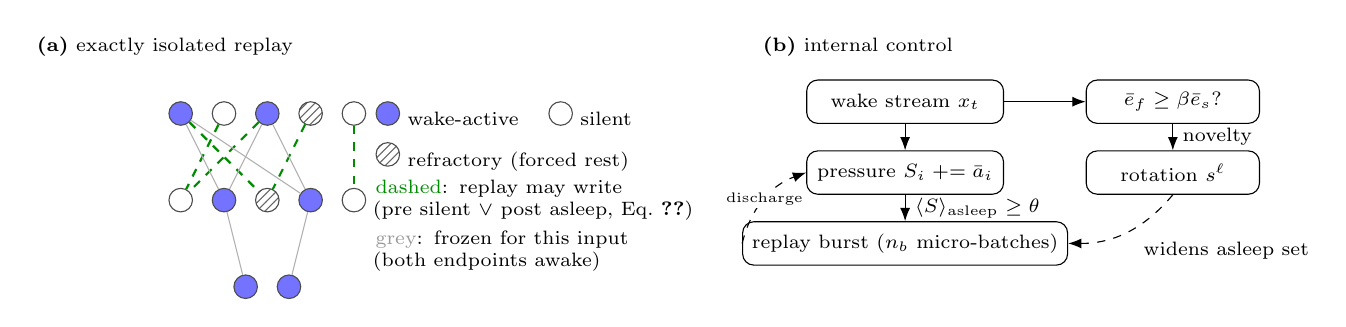
\begin{tikzpicture}[
  font=\scriptsize, >=Latex,
  unit/.style={circle, draw=black!70, minimum size=8.5pt, inner sep=0pt},
  awake/.style={unit, fill=blue!55},
  asleep/.style={unit, fill=white},
  refr/.style={unit, pattern=north east lines, pattern color=black!60},
  lay/.style={},
]
% ---- panel (a): isolation rule
\node at (-0.2,3.05) {\textbf{(a)} exactly isolated replay};
\foreach \i/\st in {0/awake,1/asleep,2/awake,3/refr,4/asleep}
  \node[\st] (x\i) at (0.55*\i, 2.2) {};
\foreach \i/\st in {0/asleep,1/awake,2/refr,3/awake,4/asleep}
  \node[\st] (h\i) at (0.55*\i, 1.1) {};
\foreach \i/\st in {1/awake,3/awake} \node at (0.55*\i, 0.0) {};
\node[awake] (o0) at (0.825, 0.0) {};
\node[awake] (o1) at (1.375, 0.0) {};
% allowed replay synapses (pre silent or post asleep): dashed green
\draw[green!55!black, dashed, thick] (x1) -- (h0);
\draw[green!55!black, dashed, thick] (x3) -- (h2);
\draw[green!55!black, dashed, thick] (x4) -- (h4);
\draw[green!55!black, dashed, thick] (x2) -- (h0);
\draw[green!55!black, dashed, thick] (x0) -- (h2);
% frozen synapses (both awake): grey
\draw[black!30] (x0) -- (h1); \draw[black!30] (x2) -- (h1);
\draw[black!30] (x0) -- (h3); \draw[black!30] (x2) -- (h3);
\draw[black!30] (h1) -- (o0); \draw[black!30] (h3) -- (o1);
\node[align=left, anchor=west] at (2.35, 2.2)
  {\tikz\node[awake]{}; wake-active \quad \tikz\node[asleep]{}; silent};
\node[align=left, anchor=west] at (2.35, 1.65)
  {\tikz\node[refr]{}; refractory (forced rest)};
\node[align=left, anchor=west, text width=4.3cm] at (2.35, 1.1)
  {\textcolor{green!55!black}{dashed}: replay may write\\ (pre silent $\lor$ post asleep, Eq.~\ref{eq:mask})};
\node[align=left, anchor=west, text width=4.3cm] at (2.35, 0.45)
  {\textcolor{black!40}{grey}: frozen for this input\\ (both endpoints awake)};
% ---- panel (b): control loop
\begin{scope}[xshift=8.0cm]
\node at (0.6,3.05) {\textbf{(b)} internal control};
\node[draw, rounded corners, minimum width=2.5cm, minimum height=0.55cm] (wake) at (1.2, 2.35) {wake stream $x_t$};
\node[draw, rounded corners, minimum width=2.5cm, minimum height=0.55cm] (press) at (1.2, 1.45) {pressure $S_i \mathrel{+}= \bar a_i$};
\node[draw, rounded corners, minimum width=2.5cm, minimum height=0.55cm] (burst) at (1.2, 0.55) {replay burst ($n_b$ micro-batches)};
\node[draw, rounded corners, minimum width=2.2cm, minimum height=0.55cm] (nov) at (4.6, 2.35) {$\bar e_f \ge \beta \bar e_s$?};
\node[draw, rounded corners, minimum width=2.2cm, minimum height=0.55cm] (rot) at (4.6, 1.45) {rotation $s^\ell$};
\draw[->] (wake) -- (press);
\draw[->] (press) -- node[right]{$\langle S\rangle_{\mathrm{asleep}} \ge \theta$} (burst);
\draw[->, dashed] (burst.west) to[bend left=28] node[fill=white, inner sep=1pt]{\tiny discharge} (press.west);
\draw[->] (wake.east) -- (nov.west);
\draw[->] (nov) -- node[right]{novelty} (rot);
\draw[->, dashed] (rot.south) to[bend left=25] node[below right]{\ widens asleep set} (burst.east);
\end{scope}
\end{tikzpicture}
\caption{\textbf{Mechanism.} (a) During each waking batch, replay from the episodic buffer is
written only into synapses whose update is invisible to the current input --- exactly so for
silent presynaptic and suppressed units (Propositions~\ref{prop:pre}--\ref{prop:post});
refractory rotation forces recently used units
into the consolidable set (Corollary~\ref{cor:refr}). (b) Two internal signals: unit-level
homeostatic pressure triggers replay bursts; a relative-novelty gate decides when rotation runs. The default system runs rotation always on and replays one micro-batch at every
waking batch; the pressure trigger and the novelty gate are the schedulers studied under
sparse replay budgets and lower activity fractions.}
\label{fig:mech}
\end{figure}

\begin{figure}[t]
\centering
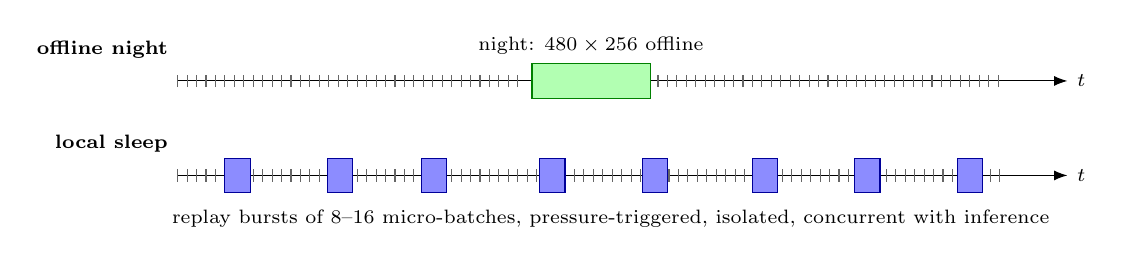
\begin{tikzpicture}[font=\scriptsize, >=Latex]
% timeline comparison
\draw[->] (0,1.5) -- (11.3,1.5) node[right]{$t$};
\node[left] at (0,1.9) {\textbf{offline night}};
\foreach \x in {0,0.12,...,4.4} \draw[black!60] (\x,1.42) -- (\x,1.58);
\draw[fill=green!30, draw=green!50!black] (4.5,1.28) rectangle (6.0,1.72);
\node at (5.25,1.95) {night: $480 \times 256$ offline};
\foreach \x in {6.1,6.22,...,10.5} \draw[black!60] (\x,1.42) -- (\x,1.58);
\draw[->] (0,0.3) -- (11.3,0.3) node[right]{$t$};
\node[left] at (0,0.7) {\textbf{local sleep}};
\foreach \x in {0,0.12,...,10.5} \draw[black!60] (\x,0.22) -- (\x,0.38);
\foreach \x in {0.6,1.9,3.1,4.6,5.9,7.3,8.6,9.9} \draw[fill=blue!45, draw=blue!60!black] (\x,0.08) rectangle (\x+0.32,0.52);
\node at (5.5,-0.25) {replay bursts of $8$--$16$ micro-batches, pressure-triggered, isolated, concurrent with inference};
\end{tikzpicture}
\caption{\textbf{Consolidation schedules.} Ticks are waking batches. The offline night pauses the
stream; local sleep consolidates during it, in replay bursts confined to asleep units.}
\label{fig:timeline}
\end{figure}

\begin{figure}[h]
\centering
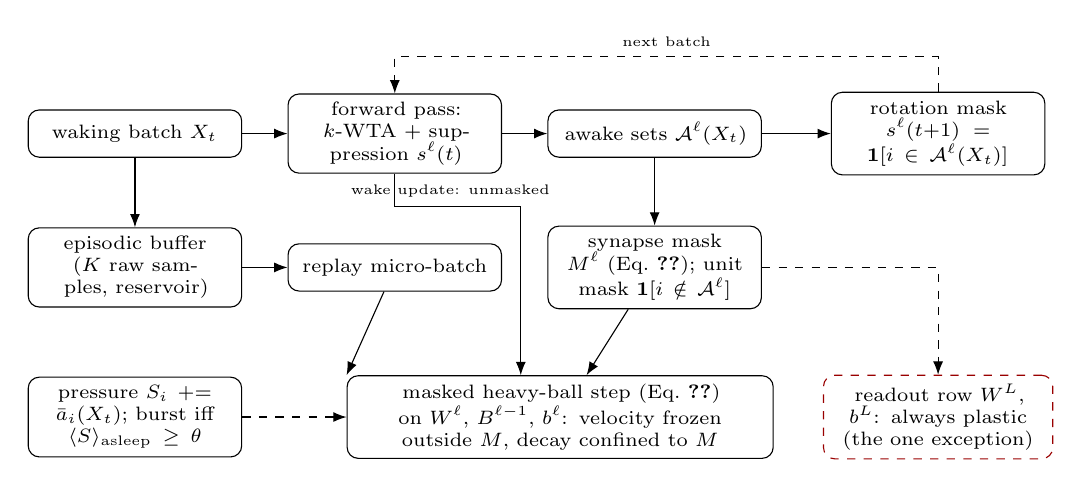
\begin{tikzpicture}[font=\scriptsize, >=Latex,
  box/.style={draw, rounded corners, inner sep=3pt, align=center, minimum height=6mm, text width=2.5cm},
  wide/.style={box, text width=5.2cm},
  exc/.style={box, dashed, draw=red!60!black, text width=2.7cm}]
\node[box] (wake)  at (0,0)     {waking batch $X_t$};
\node[box] (fwd)   at (3.3,0)   {forward pass: \kwta{} $+$ suppression $s^\ell(t)$};
\node[box] (awake) at (6.6,0)   {awake sets $\mathcal{A}^\ell(X_t)$};
\node[box] (rot)   at (10.2,0)  {rotation mask $s^\ell(t{+}1)=\mathbf{1}[i\in\mathcal{A}^\ell(X_t)]$};
\node[box] (buf)   at (0,-1.7)  {episodic buffer ($K$ raw samples, reservoir)};
\node[box] (rep)   at (3.3,-1.7){replay micro-batch};
\node[box] (mask)  at (6.6,-1.7){synapse mask $M^\ell$ (Eq.~\ref{eq:mask}); unit mask $\mathbf{1}[i\notin\mathcal{A}^\ell]$};
\node[box] (press) at (0,-3.6)  {pressure $S_i \mathrel{+}= \bar a_i(X_t)$; burst iff $\langle S\rangle_{\mathrm{asleep}}\ge\theta$};
\node[wide](step)  at (5.4,-3.6){masked heavy-ball step (Eq.~\ref{eq:maskedstep}) on $W^\ell$, $B^{\ell-1}$, $b^\ell$: velocity frozen outside $M$, decay confined to $M$};
\node[exc] (ro)    at (10.2,-3.6){readout row $W^L$, $b^L$: always plastic (the one exception)};
\draw[->] (wake) -- (fwd); \draw[->] (fwd) -- (awake); \draw[->] (awake) -- (rot);
\draw[->] (awake) -- (mask); \draw[->] (mask) -- (step);
\draw[->] (buf) -- (rep); \draw[->] (rep) -- (step.north west);
\draw[->] (wake) -- (buf);
\draw[->] (fwd.south) -- ++(0,-0.42) -| node[pos=0.22, above, font=\tiny]{wake update: unmasked} ([xshift=-0.5cm]step.north);
\draw[->, dashed] (press) -- (step);
\draw[->, dashed] (rot.north) |- ++(0,0.45) -| node[pos=0.25, above, font=\tiny]{next batch} (fwd.north);
\draw[->, dashed] (mask.east) -| (ro.north);
\end{tikzpicture}
\caption{\textbf{Training data flow.} Each waking batch is inferred under the current
suppression mask; its awake sets define the synapse and unit masks for the replay micro-batch
applied in the same step and the rotation mask for the next batch. The masked step confines
the velocity and the decay to the mask; the readout row is the one deliberately plastic
exception. Unit-level pressure decides when replay bursts run.}
\label{fig:dataflow}
\end{figure}

\subsection{Cost accounting}

\paragraph{Updates and wall-clock.} Samples are not the only cost: the headline schedule makes
$18{,}760$ masked updates against the night's $480$ ($39\times$), and its training wall-clock
on one CPU is $6.6$ min against $0.6$ for the night, $0.4$ with no replay and $6.0$ for
unmasked interleaved replay --- the per-batch replay step, not the sample count, is the online
price of consolidating during the stream, in an unoptimised implementation whose mask
construction is dense.
\paragraph{Baseline tuning and paired comparison.} The offline-night reference was swept over
replay batch count ($20$, $40$ per night), replay batch size ($16$, $64$, $256$), learning-rate
gain ($3\times$), core width ($256$--$128$ and $512$--$256$), buffer size ($200$, $1000$,
$5000$) and timing (clocked after each epoch, novelty-timed, surprise-timed), and its best
sequential cell is reported; BP+ER was swept over learning rate ($3{\cdot}10^{-4}$,
$10^{-3}$, $3{\cdot}10^{-3}$), width and buffer size; the local learner over $\eta$
(Appendix~\ref{app:eta}), replay batch size, cadence and the gates of
Table~\ref{tab:ablation}. Selection everywhere was sequential accuracy at
$K{=}1000$ with the static axis reported alongside, on the official test set, which served as
the development set; the numbers reported are on the held-out split (Appendix~\ref{app:val}).
Pairing seeds by index on that split, the local system's margin over the narrow-substrate
night is $+2.5$ points (bootstrap 95\% CI $[+1.3,+4.8]$, three seed pairs), over the
same-substrate night $+2.6$ ($[+0.2,+5.2]$, six pairs; the night's seed variance makes this
one fragile, and on the second split it shrinks to $+0.3$), over unmasked interleaved ER
$+6.3$ ($[+3.8,+9.2]$), over BP+ER $+2.8$ ($[+2.5,+3.2]$), over the silent mask $+3.6$
($[+3.1,+4.1]$) and over rotation alone $+0.1$ ($[-0.3,+0.5]$).
Replay cost is measured in samples ($R_s$ = batches $\times$ batch size) and synaptic work.
The night costs $R_s = 480\times256 \approx 1.2\times10^5$ samples. The headline configuration (one $16$-sample micro-batch per waking batch, $91.6\pm0.3$) costs
$18{,}760\times16\approx3.0\times10^5$ samples ($2.4\times$ the night). Two schedules meet
the night's budget within $1.2\times$: eight-sample micro-batches at every waking batch ($1.5\times10^5$, $91.1\pm0.4$) and $16$-sample
micro-batches at every second one ($1.5\times10^5$, $91.2\pm0.2$ sequential, $93.1\pm0.2$
static); pressure-triggered bursts of $16$ at a third of the events reach $88.6\pm1.6$. Accuracy is bought by
the frequency of small isolated updates rather than by replayed samples.

% ---------------------------------------------------------------- 5
\section{Results}
\label{sec:results}

\subsection{Local sleep replaces the night}
\label{sec:r1}

On split-MNIST at $K{=}1000$, refractory local sleep with an isolated replay micro-batch
beside every waking batch reaches $\mathbf{91.6\pm0.3\%}$ (six seeds) with no offline phase
--- above the best offline night ($89.2\pm1.7\%$ on the night's preferred narrow substrate;
$89.0\pm3.5$, highly variable across seeds, on ours; paired margins $+2.5$ $[+1.3,+4.8]$ and
$+2.6$ $[+0.2,+5.2]$), above unmasked interleaved ER at the same budget ($87.5\pm0.8$ under
Adam, $85.4\pm3.5$ under SGD) and above BP+ER ($88.8\pm0.3$; $+2.8$ $[+2.5,+3.2]$). Halving
the cadence with $16$-sample batches costs $0.4$ ($91.2\pm0.2$). Adding a night on top of
continuous local sleep adds $0.8$ ($92.4\pm0.3$ vs.\ $91.6\pm0.3$): once consolidation runs
during wake, the offline phase is nearly redundant at this buffer size. At very small buffers
($K{=}200$) the night retains an edge only in combination with narrow substrates; the
mechanism triangulation is in Appendix~\ref{app:k200}.

\paragraph{A second split.} On a second, independent held-out tenth the ordering holds
(rotation $91.8\pm0.4$, BP+ER $88.5\pm0.7$, unmasked ER $80.0\pm14.1$, the narrow night
$89.3\pm0.6$, the silent mask $88.6\pm1.3$, rotation alone $91.8\pm0.6$), with one exception
worth stating: the same-substrate night, bimodal on the first split, reaches $91.5\pm0.5$ on
the second and trails by only $0.3$ there (Appendix~\ref{app:val}).

\subsection{What rotation and isolation each buy}
Figure~\ref{fig:batch}: the full system is flat in replay batch size from $256$ down to $8$
samples ($91.6\pm0.5\to91.1\pm0.4$) and loses $1.9$ at $4$ ($89.7\pm0.7$), while at batch $16$
unmasked replay without rotation sits at $85.4\pm3.5$, isolation without rotation at
$88.0\pm0.7$, and the offline night falls from $89.0$ to $85.8\pm3.0$ when its batches shrink
to $16$. The fourth cell of the square --- rotation with unmasked replay --- reaches
$91.5\pm0.3$ at batch $16$, $90.9\pm0.1$ at $8$ and $89.3\pm0.7$ at $4$: the two factors are
strongly sub-additive, rotation is the larger single factor ($+6.1$ alone, $+3.6$ on top of
isolation), and isolation's seed-paired margin is $0.1$ $[-0.3,+0.5]$ at batch $16$, $0.3$
$[-0.2,+0.6]$ at $8$ and $0.3$ $[-0.5,+1.2]$ at $4$ --- within seed noise at every size --- with
$0.4$ on the static axis ($94.1$ vs.\ $93.7$). At two-sample batches both systems lose
heavily, but differently: isolated replay degrades gracefully ($79.0\pm3.2$, six seeds within
$75$--$84$), whereas unmasked replay bifurcates --- three seeds at $82$--$85$, one at $58$ and
two at chance (Appendix~\ref{app:isomargin}). Isolation's accuracy value is thus not a margin
but the removal of a failure mode; what it buys at every batch size is the guarantee that,
for the current input under its suppression mask, replay leaves the hidden activities
unchanged --- exactly on the proven channels, within the margin elsewhere; without it every
micro-batch perturbs the live coalition and the outcome rests on the rotation's tolerance of
that perturbation, which runs out at batch $2$. The earlier ``$39\times$'' cost of inference-time consolidation was an artefact
of counting $256$-sample batches.

\begin{figure}[t]
\centering
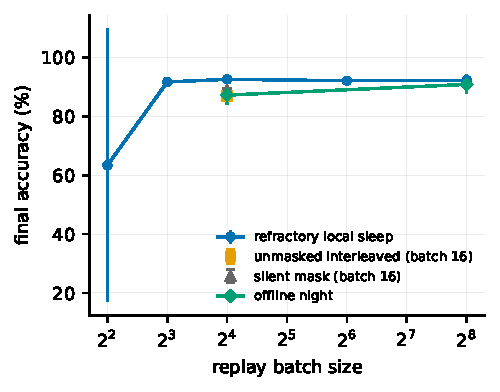
\includegraphics[width=.48\linewidth]{figs/fig_batch.pdf}\hfill
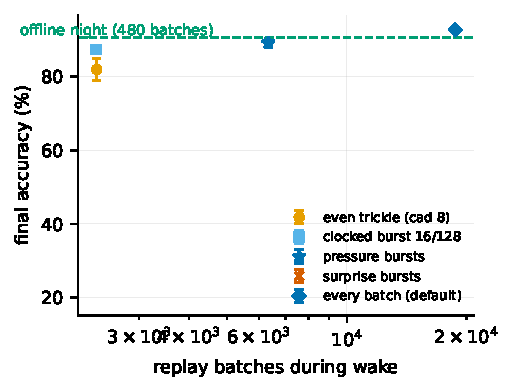
\includegraphics[width=.48\linewidth]{figs/fig_timing.pdf}
\caption{\textbf{Left (isolation):} final split-MNIST accuracy vs.\ replay batch size
(record substrate, heavy-ball SGD); the number of updates is fixed within each series (one per
waking batch; $20$ per epoch for the night, whose samples therefore fall with its batch).
The full system is flat down to $8$ samples and loses $1.9$ at $4$ ($12.7$ at $2$,
Appendix~\ref{app:isomargin}); rotation with unmasked replay (dashed) trails it by $0.1$ to
$0.3$, within seed noise, and collapses in half the seeds at batch $2$; without rotation,
unmasked and isolated replay and the offline night all degrade. \textbf{Right
(timing):} accuracy vs.\ number of waking replay batches. Trickles and clocked bursts fail alike; pressure-triggered bursts (star) keep most of the
accuracy at a third of the events; surprise triggering fires no events in this regime.}
\label{fig:batch}
\end{figure}

\subsection{The direction of protection matters, and the least optimiser state suffices}
\label{sec:direction}
Two ablations sharpen the construction. \emph{Mirror isolation} implements the classical
protected direction with our own machinery: the \emph{waking} update is barred from synapses
whose both endpoints served the last replay batch (protect the past), while replay itself is
applied unmasked. With everything else identical, mirror isolation reaches only $78.0\pm3.2\%$ --- below even
unmasked interleaved ER ($87.5\pm0.8$ under Adam) and far below our direction ($91.6\pm0.3$): constraining wake learning impairs the new task while the unmasked replay keeps
perturbing the live computation, a double loss. This reversed-mask control thus loses fourteen points ($20$, with high seed variance
$70.3\pm10.1$, at the historical $5\%$ fraction, development phase); it is one instantiation of the
protect-the-past direction, not a verdict on that literature. (An earlier version of this cell ran with
the burst-rate baseline inadvertently frozen during the masked waking update and read
$85.0\pm2.0$; the corrected cell shares its bookkeeping with every other row.)
Second, replacing masked Adam with heavy-ball SGD --- a single per-synapse velocity, no
second-moment state --- inside the same isolation gives $\mathbf{91.6\pm0.3\%}$ sequential and
$94.1\pm0.2\%$ static (six seeds), a tie with masked Adam ($91.5\pm0.4/94.1\pm0.1$; unmasked
SGD control $85.4\pm3.5$). Carrying a single velocity and nothing else is simpler at equal
accuracy --- and closer to biology; carrying \emph{nothing} is not: with momentum zero the isolated replay micro-batches lose the
velocity's noise averaging, activity collapses to chance at every learning rate unless the
replay step is re-scaled by hand, and the best pure-SGD setting then trails by $3.2$ sequential and $4.7$ static points
($88.4\pm0.5/89.4\pm0.3$). The ablation in Section~\ref{sec:ablation} finds no deficit to trace on the held-out split:
confined and leaking moments tie, so the confinement of the update over time comes free. Third, \emph{soft} rotation (halving, rather than silencing, recent winners) loses where it
matters ($89.9\pm0.7$ sequential, $84.3\pm1.0$ static): all-or-none OFF periods beat turned-down
gain, echoing the biological finding that tonic firing-rate reduction does not discharge local
sleep pressure while ON/OFF alternation does \citep{driessen2026}. Table~\ref{tab:ablation} in
Section~\ref{sec:ablation} collects these controls together with the remaining component
knockouts; a two-sided learning-rate sweep (Appendix~\ref{app:eta}) shows the comparison is a
plateau rather than a knife-edge, with masked Adam already at its own best.

\subsection{When replay must be rare: homeostatic bursts, not surprise}
Figure~\ref{fig:batch} (right): at $12.5\%$ of replay events, a clocked burst of $16$ batches every $128$ reaches $80.5\pm6.1$, no better than an even
trickle at the same budget ($78.5\pm2.6$). Unit-level pressure triggering keeps
$88.6\pm1.6$ at a third of the events, and surprise triggering fails: at the record fraction the converged error never
crosses the surprise threshold, so \emph{zero} replay events fire ($18.8$, the forgetting floor). Homeostatic triggering consistently outperforms the tested surprise trigger during
wake --- the opposite of the night, whose best trigger in our sweeps is novelty-timed. (The
same ordering held throughout the historical $5\%$ phases, where the surprise trigger fired
occasionally and still failed at every volume.)

\subsection{The i.i.d.\ price of rotation}
Rotation's i.i.d.\ price depends on the activity fraction. At the historical $5\%$ it cost
$1.5$ points on i.i.d.\ MNIST ($92.6$ vs.\ $94.1$ rotation-free; $1.3$--$3.0$ across the
development-phase gate grids) and, in development, \emph{reversed} into a $+2.5$ to
$+6.5$-point static gain on split CIFAR-10 (forced rotation as a regulariser in the underfit
regime); at the $10\%$ record fraction the MNIST price is $1.2$--$1.7$ points ($94.1$ vs.\
$95.3$--$95.8$ rotation-free) and the CIFAR static effect is inconclusive under the available
seeds ($28.0\pm1.2$ vs.\ $30.0\pm1.9$). Under masked Adam, a relative-novelty/progress gate
(Eqs.~\eqref{eq:nov}--\eqref{eq:prog}) removed the $5\%$ price with one setting across all
four regimes; the full Adam-era gate study --- including why a single absolute threshold cannot serve across the regimes considered here and why unit-level pressure gating only trades the axes --- is in
Appendix~\ref{app:gates}. Under heavy-ball SGD the gate had to be committed to bouts
(Section~\ref{sec:ablation}); at the record fraction both cures become largely unnecessary
--- the sparsity dial (Section~\ref{sec:dial}) shrinks the price at source.

\subsection{Transfer to CIFAR-10}
On split CIFAR-10 (grayscale, same protocol) the ordering transfers and widens: refractory local sleep $28.9\pm1.0$ $>$ offline night $25.7\pm1.2$ $>$ BP+ER $24.8\pm0.3$ $>$
unmasked ER $15.4\pm4.2$ $\approx$ no buffer $16.3$ (the same on the second split:
$29.7>26.5>25.8>15.5$), despite task-active code overlap of $0.9$--$0.98$. On the V1-like feature front-end the local ordering persists (refractory $42.3\pm0.6$ $>$ offline night $34.0\pm0.8$ $\gg$ unmasked $20.5\pm1.0$) and BP+ER
reaches $42.8\pm0.7$ at its best learning rate --- the reverse of the
raw-pixel ordering. At the $5\%$ fraction of the earlier phases (local learner at $36.8$, development phase)
this was a $4.7$-point regime boundary; a two-sided fairness pass plus the sparsity dial
revise it to $0.5$ ($42.3\pm0.6$ local vs.\ $42.8\pm0.7$ BP+ER): most of the
boundary was the local learner's optimiser and its starved activity fraction, not its
learning rule. On raw pixels the local learner leads outright.

The tested decomposition is consistent with the \emph{substrate}, not the learning rule,
accounting for the residual mean gap.
Transplanting the local network's ingredients into the BP net one at a time (each cell at its
better of two learning rates): its width \emph{helps} BP+ER ($43.7\pm1.0$ for a dense $512$--$256$ net), its $30\%$
distance-dependent wiring --- drawn by the same generator on the same sheets --- is neutral
($43.5\pm0.2$), and its \kwta{} costs $3$ points ($40.4\pm1.5$ at the record $10\%$;
$39.5\pm0.6$ at $5\%$), leaving backprop-with-replay \emph{below} the local learner on the
identical substrate ($42.3\pm0.6$ vs.\ $40.4\pm1.5$ at $10\%$; three seeds each). What separates the
two systems on feature inputs is dense activation, not backpropagation's credit assignment: on
the substrate used here, the tested decomposition leaves no gap attributable to the learning
rule. The advantage over
\emph{other local schedules} (nights, unmasked ER) remains robust across all three input
regimes.


\subsection{Energy}
Converted to spiking inference ($T_s{=}8$; firing thresholds calibrated on training images,
evaluated on the held-out tenth), the default system (always-on rotation, heavy-ball SGD,
record fraction; rate accuracy $94.2\%$ on the measured seed) runs at $92.7\%$ and
$117$\,nJ/sample vs.\ $2461$\,nJ for dense rate inference ($21\times$) and $526$\,nJ for
event-driven rate inference ($4.5\times$), improving with the time budget ($94.0\%$ at
$T_s{=}16$, $236$\,nJ; $94.0\%$ at $T_s{=}32$). The rotation-free control converts to
$94.2\%$ at $T_s{=}8$ and dips to $93.9\%$ at $T_s{=}32$; the calibration interaction we had
reported under the Adam stack (the rotation-free control degrading sharply with $T_s$) does
not reproduce at this magnitude under heavy-ball SGD on the held-out split.

\subsection{Negative results}
For the record, the following were falsified under matched budgets: a frozen dentate-gyrus-style
sparse expansion front-end (input decorrelation does not propagate through learned \kwta{} layers:
task overlap at the input drops $0.79\to0.18$ yet every downstream metric worsens by $3$--$11$
points); generative (REM) replay as a substitute for episodic samples; margin-based reverse
learning; surprise-gated memory \emph{writing}; multiplicative burst coding; absolute-threshold
rotation gates; pruning anchored to sparse replay bursts (Appendix~\ref{app:downsel}); soft (gain-reduction) rotation
and mirror-direction isolation (Section~\ref{sec:direction}); an OFF-side gate refractory ---
the flip-flop's inactive half in this system; strongly coupled synaptic anchors; and
utility-exempt rotation as a route past the bout gate (all Section~\ref{sec:ablation}).

% ---------------------------------------------------------------- 5b
\section{Ablation Study}
\label{sec:ablation}

The system under test is a conjunction of five ingredients: a biologically constrained
substrate, the exact isolation mask \eqref{eq:mask}, the refractory rotation, a heavy-ball
optimiser, and the progress-keyed gate \eqref{eq:prog}. This section removes or replaces one ingredient of the consolidation mechanism at a time
(Table~\ref{tab:ablation}). The substrate beneath it was fixed by earlier ablation ladders;
its full cost accounting --- $1.2$ points below a dense backpropagation MLP at $4\times$
fewer synaptic operations per pass --- is reproduced in Appendix~\ref{app:substrate}. Every
mechanism cell shares the record substrate ($512$--$256$ hidden, $10\%$ \kwta{}, $30\%$
distance-dependent connectivity), the same buffer ($K{=}1000$, random writing) and the same
replay budget (waking batch $16$, replay batch $16$ after every waking batch); the appendices
retain the corresponding grids at the historical $5\%$ fraction, where every ordering below
was first established.

\begin{table}[t]
\centering
\caption{\textbf{Component ablation of the consolidation mechanism} on the record substrate
($512$--$256$/$10\%$; backprop references dense $256$--$128$). Sequential $=$ final accuracy
on split-MNIST; static $=$ i.i.d.\ MNIST (the axis that must not degrade). Dashes:
combination not applicable. Held-out split; headline rows carry six seeds, the rest three.}
\label{tab:ablation}
\small
\begin{tabular}{@{}lcc@{}}
\toprule
Variant & Sequential & i.i.d.\ (static) \\
\midrule
\textbf{full system}: isolated replay $+$ always-on rotation (heavy-ball SGD) & $\mathbf{91.6\pm0.3}$ & $94.1\pm0.2$ \\
\quad rotation gated by relative novelty, committed to bouts & $91.8\pm0.3$ & $94.4\pm0.3$ \\
\quad rotation gated per batch & $87.5\pm1.6$ & $94.7\pm0.1$ \\
$+$ two-timescale anchor ($\lambda{=}\mu{=}3{\cdot}10^{-4}$), rotation always on & $91.7\pm0.0$ & $93.8\pm0.3$ \\
$-$ rotation (same mask, Eq.~\ref{eq:mask}, natural silence only) & $88.0\pm0.7$ & $95.3\pm0.2$ \\
$-$ isolation, $-$ rotation (unmasked interleaved replay) & $85.4\pm3.5$ & $95.8\pm0.3$ \\
$-$ isolation, $+$ rotation (rotation alone) & $91.5\pm0.3$ & $93.7\pm0.3$ \\
readout-only replay (hidden layers take no replay update) & $41.7\pm10.9$ & $82.7\pm0.3$ \\
random rotation (matched suppression count) & $91.0\pm0.8$ & $92.1\pm0.2$ \\
$-$ replay (no buffer) & $19.4\pm0.0$ & $95.1\pm0.0$ \\
\midrule
masked Adam, moments confined to the mask & $91.5\pm0.4$ & $94.1\pm0.1$ \\
masked Adam, moments leaking outside the mask & $91.6\pm0.6$ & $94.0\pm0.3$ \\
momentum $0$ (pure SGD; $\eta$ and replay gain re-tuned, else chance) & $88.4\pm0.5$ & $89.4\pm0.3$ \\
\midrule
offline night instead of concurrent replay, same substrate & $89.0\pm3.5$ & --- \\
\quad the same night on its preferred narrow substrate & $89.2\pm1.7$ & --- \\
mirror direction: protect the past & $78.0\pm3.2$ & $91.7\pm0.6$ \\
soft rotation: gain $0.5$ instead of $0$ & $89.9\pm0.7$ & $84.3\pm1.0$ \\
\midrule
unmasked ER at the same budget (Adam) & $87.5\pm0.8$ & $95.1\pm0.2$ \\
backprop ($+$ER sequential; plain static), dense & $88.8\pm0.3$ & $97.4\pm0.1$ \\
\bottomrule
\end{tabular}
\end{table}

\subsection{Reading the component table}
Read top-down, the first block prices each ingredient by what its removal costs the
sequential axis under heavy-ball SGD: rotation is worth $+3.6$ points ($91.6$ vs.\ $88.0$
for the same mask on natural silence alone), rotation and isolation together $+6.2$ with a
twelve-fold smaller seed deviation ($91.6\pm0.3$ vs.\ $85.4\pm3.5$), isolation alone $+2.6$
($88.0$ vs.\ $85.4$), isolation on top of rotation $+0.1$ ($91.5\pm0.3$ for rotation with
unmasked replay; $[-0.3,+0.5]$ paired), and replay is worth everything ($19.4$ is the
forgetting floor). Replay confined to the readout row, hidden layers frozen for replay, falls
to $41.7\pm10.9$ (ten classes) and costs $11$ static points: readout-only replay cannot
account for the full system's accuracy, and hidden-layer replay updates are essential to it.
A random suppression of matched size in place of the refractory rule recovers most of
rotation's gain ($91.0\pm0.8$) but trails it by $0.6$ sequential and $2.0$ static points with
$1.4\times$ the forgetting ($F{=}8.7$ vs.\ $6.4$): alternating the coalition carries most of
the effect, resting the recent winners the rest. The static column identifies who pays:
rotation is the only statically costly component ($94.1$ always-on against $95.3$--$95.8$
without it, and $93.7$ with rotation and no isolation), a price of $1.2$--$1.7$ points at the
record fraction. The unmasked control is not handicapped by the replay step ($3\eta$ against
a waking step of $\eta/16$): sweeping the replay gain over $\{1/16,1/4,1,3,10\}$ moves masked
replay $67.2\to86.8\to90.8\to91.6\to74.2$ and unmasked replay
$61.6\to81.4\to85.7\to85.4\to47.3$ (sequential; three seeds, six at gain $10$, where both
destabilise) --- both peak at the default and the rotation-free unmasked control never
closes the gap; the sweep bounds that control, it does not estimate isolation's own
contribution (the square above does). The gates that were built to refund a larger price at the
historical $5\%$ fraction are here \emph{neutral}: the bout-committed gate trades $+0.2$ sequential for $+0.3$ static
($91.8\pm0.3/94.4\pm0.3$), the per-batch gate is erratic ($87.5\pm1.6/94.7\pm0.1$), and the
two-timescale anchor no longer adds anything ($91.7\pm0.0/93.8\pm0.3$). Their mechanisms remain instructive --- at $5\%$ the per-batch
gate's flicker destroyed heavy-ball SGD's gain, episode commitment (loosely modelled on the
consolidated bouts of the sleep--wake switch \citep{saper2005}, which motivates commitment but
not the specific minimum duration) repaired it, and bout-length and OFF-refractory
controls located the residual price in the rotation of settled coalitions itself --- and that
full study is preserved in Appendix~\ref{app:probes} and the $5\%$ grids; but at the record
fraction the dial has absorbed most of what they bought, and the default system is simply
always-on rotation.

The middle block tests the confinement requirement itself. Propositions~\ref{prop:pre}--\ref{prop:post} require Adam's moments to advance
only inside the mask: state advancing outside re-injects the replay gradient into awake
synapses through the next unmasked waking step: the present batch's invariance still holds,
since the weight change itself stays masked, but the confinement of the update over time is
lost. Empirically, on the held-out split, confined and leaking moments tie ($91.5\pm0.4$ vs.\
$91.6\pm0.6$), as does the single velocity ($91.6\pm0.3$): in development the leak had
appeared to help by $0.8$, a margin that did not survive the protocol change. The velocity is
kept as the least state that stays confined to the mask at equal accuracy: it advances only
inside the mask, and removing it as well (momentum zero, Table~\ref{tab:ablation}) costs
$3.2$/$4.7$ points once the replay step has been re-scaled to survive at all.

One budget note completes the block: half the cadence with $16$-sample batches costs $0.4$
($91.2\pm0.2$) --- the system prefers consolidation to run continuously.

\subsection{Two probes of the residual static price}
At the historical $5\%$ fraction, the OFF-refractory null located the bout gate's residual
static price in the rotation of settled coalitions itself. Two mechanisms attacked that
diagnosis directly (details in Appendix~\ref{app:probes}; $5\%$ numbers).
\emph{Utility-exempt rotation} (sparing the top-$q$ long-use units from ever being benched)
only traces a trade-off that the bout gate dominates: temporal commitment beats structural
exemption. \emph{Two-timescale synapses} in the spirit of synaptic consolidation cascades
\citep{benna2016} fail to dissolve the price, but weak symmetric coupling acts as a
\emph{sequential stabiliser} at $5\%$ ($92.4\pm0.2$, variance halved, static parity); at the record fraction the anchor is neutral ($91.7\pm0.0/93.8\pm0.3$). Anchor and bout gate
compose sub-additively. Figure~\ref{fig:frontier} draws the operating frontier.

\begin{figure}[t]
\centering
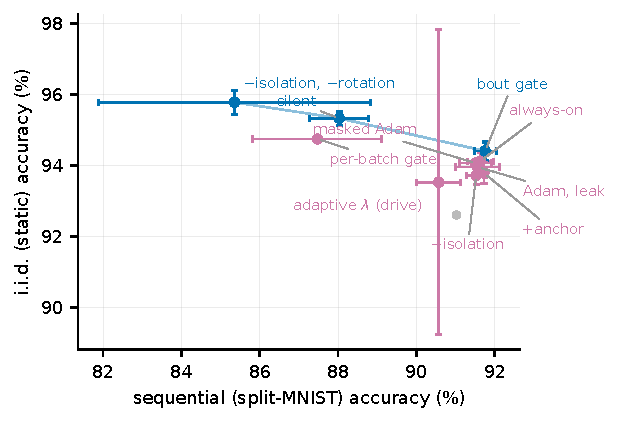
\includegraphics[width=.6\linewidth]{figs/fig_frontier.pdf}
\caption{\textbf{The operating frontier} at the record fraction under heavy-ball
SGD: split-MNIST sequential accuracy against i.i.d.\ static accuracy (headline points
six seeds). Blue: non-dominated configurations; purple: dominated ones; held-out split. The adaptive-$\lambda$ point (Section~\ref{sec:controller}) sits on the static
side of the frontier. No single configuration wins both
axes; always-on rotation is the sequential default.}
\label{fig:frontier}
\end{figure}

\begin{figure}[h]
\centering
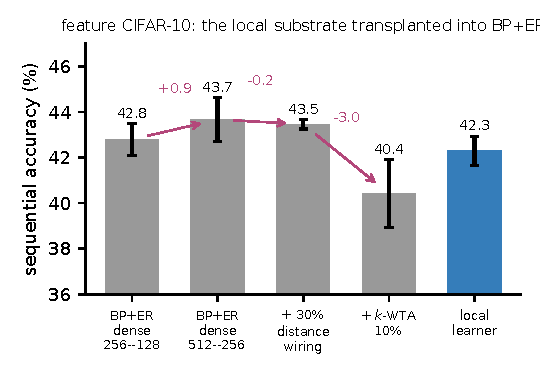
\includegraphics[width=.48\linewidth]{figs/fig_waterfall.pdf}\hfill
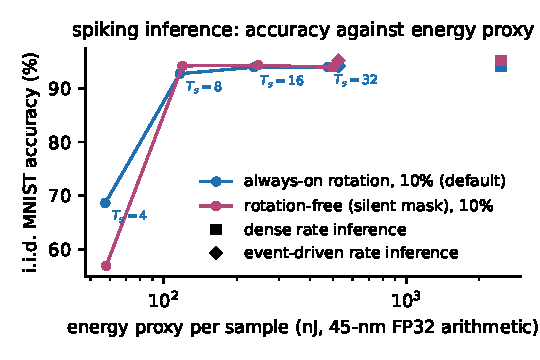
\includegraphics[width=.48\linewidth]{figs/fig_pareto.pdf}
\caption{\textbf{Left:} the substrate decomposition on feature CIFAR-10 --- transplanting the
local network's ingredients into BP+ER one at a time (each cell at its better of two learning
rates; six seeds except the local learner, three). \textbf{Right:} spiking inference,
i.i.d.\ MNIST accuracy against the idealised 45-nm FP32 arithmetic-energy proxy for
$T_s\in\{4,8,16,32\}$, with the dense (square) and event-driven (diamond) rate references;
held-out split; the default is monotone in $T_s$, the rotation-free control dips $0.4$ at
$T_s{=}32$.}
\label{fig:appfigs}
\end{figure}

\subsection{The sparsity dial}
\label{sec:dial}
The substrate's original $5\%$ \kwta{} fraction was fixed in an early phase and inherited by
a year of experiments; the decomposition just given made it suspect --- if sparse \kwta{}
taxes BP by points on features, it presumably taxes our own learner too. It did, on both
regimes, and the tax was bought back almost for free; this subsection documents the dial that
led to the $10\%$ record fraction used throughout the main text. On feature CIFAR-10, relaxing the
fraction improves \emph{both} axes monotonically: sequential $40.9\to42.9\pm0.6$ and static $38.3\to46.4\pm1.6$ from $5$ to $25\%$, with
forgetting slightly \emph{reduced}; the BP control traces the same curve
($39.5\to40.4\to40.7$ at $5$, $10$, $15\%$), with the local learner $1.4$--$1.9$ points ahead
at every matched level. On MNIST the sequential axis is flat from $10\%$: always-on rotation
reaches $\mathbf{91.6\pm0.3}$ sequential at $94.1\pm0.2$ static (six seeds), $15\%$ gives
$91.4\pm0.4/94.4\pm0.2$ and $25\%$ $91.5\pm0.4/94.6\pm0.2$, against $91.0\pm0.5/92.6\pm0.0$ at
the historical $5\%$.

Three controls sharpen the reading. First, the no-buffer ceiling itself rises with the fraction ($94.1$ at $5\%$, $95.1$ at $10\%$),
so rotation's static price \emph{at matched sparsity} shrinks from $1.5$ to $1.0$ points ---
and the gate's raison d'\^etre shrinks with it: at $10\%$ always-on rotation no longer trails
the bout-gated system. Second, in development, rotation-free silent isolation gained nothing
from the dial ($89.0\to89.3\to88.7$, official test set): the dial helps specifically the
\emph{rotating} family, which at $5\%$ was starved of representational room. Third,
asymmetric schedules (a mild input-facing layer above a sparse deep layer) failed in
development --- sequential parity with uniform relaxation but a $3$--$4$-point static
deficit: the tax is levied at every layer. The dial is free elsewhere: synaptic operations
rise only $3$--$5\%$. Following this finding the record substrate moved to $10\%$:
Table~\ref{tab:ablation} and every main-text number now use it, with the complete mechanism
grid re-established there (orderings preserved throughout), while the appendices retain the
historical $5\%$ grids on which each mechanism was first isolated. The dial, not the gate, is
the cheapest cure for rotation's static price (Figure~\ref{fig:frontier}).

% ---------------------------------------------------------------- 6
\section{An adaptive decay controller}
\label{sec:controller}

\paragraph{The last tuned constant.}
Every result above runs the rule of \eqref{eq:kp} with a decay $\lambda$ tuned once per
dataset ($10^{-3}$ on the image benchmarks). Split CIFAR-100 --- ten tasks of ten classes ---
exposes what that constant hides. With one hundred classes, each class receives a tenth of
the per-epoch supervision events, while the decay acts on every synapse at every step,
undiminished; at the MNIST-tuned value the hidden-to-hidden weights follow the pure-decay
trajectory $(1-\lambda)^t$ \emph{exactly} (the thinned error signal loses the race outright),
deep activity collapses by $5\times$, the readout gradient goes to zero, and the network
lands at chance --- $2.4\%$ i.i.d.\ against $20$--$23\%$ for a ten-class subset of the same
images on the same substrate (development-phase diagnosis). The class count of the
supervision signal is a hidden variable that every fixed $\lambda$ is silently tuned against.
A manual rescue ($\lambda{=}10^{-4}$, $3\times$ targets) revives activity but survives the full
protocol only at $1.0$--$1.2\%$.

\paragraph{The controller.}
The project's design principle --- control signals must be self-referenced, never absolute
(Section~\ref{sec:rotation}) --- applies at the synapse. We replace the constant by a
per-layer ratio controller,
\begin{equation}
\lambda_\ell \;=\; \min\!\Big(\lambda_{\max},\; \rho\,
\frac{\mathrm{EMA}\big[\,u^\ell\,\big]}{\overline{|W^\ell|}+\epsilon}\Big),
\qquad \rho=0.25,\;\; \lambda_{\max}=0.02,
\label{eq:controller}
\end{equation}
where $u^\ell$ is the mean magnitude of the data-driven, post-optimiser, \emph{pre-decay}
waking increment applied to layer $\ell$ (so the decay never feeds its own drive), the EMA
(coefficient $0.02$) runs over waking, unmasked steps only, $\epsilon=10^{-12}$ floors the
denominator, and $W^\ell$ and $B^{\ell-1}$ share $\lambda_\ell$, so Kolen--Pollack alignment
is untouched. The decay's mean magnitude per step, $\lambda_\ell\overline{|W^\ell|}$, is held at
the fraction $\rho$ of the mean data-driven update magnitude: layers and regimes with rich
supervision keep a strong regulariser, starved ones are automatically spared. $\rho$ is the only control target; $\lambda_{\max}$, the EMA coefficient and
$\epsilon$ are global safeguards never tuned per dataset. Isolation and rotation decide
\emph{where} and \emph{when} to consolidate; the controller decides \emph{how strongly} to
update as the scale changes, by the principle behind every control signal in this paper ---
novelty as a fast-over-slow error ratio, homeostasis as a unit's own use, decay as a
drive-over-weight ratio: all referenced to the learner's own current state, none absolute. A gradient-referenced variant ($\rho\,\eta\,\mathrm{EMA}[\,\overline{|g^\ell|}\,]/
\overline{|W^\ell|}$) behaved equivalently in development (official test set, not re-run
under the held-out protocol); the drive-referenced form is canonical because it is
optimiser-agnostic.

\begin{table}[t]
\centering\small
\caption{\textbf{One dataset-independent ratio target replaces per-dataset decay tuning.} Sequential /
static accuracy (\%) under the tuned fixed decay ($10^{-3}$ on the image benchmarks;
$10^{-4}$ with $3\times$ targets as the CIFAR-100 rescue) against the drive-referenced
controller of \eqref{eq:controller} at the same $\rho=0.25$ everywhere; held-out split, three
seeds (six on split-MNIST); the full system (refractory rotation, isolated replay, $K{=}1000$)
in every cell.}
\label{tab:controller}
\begin{tabular}{lcccc}
\toprule
& \multicolumn{2}{c}{fixed $\lambda$ (tuned)} & \multicolumn{2}{c}{controller (drive)} \\
& seq. & static & seq. & static \\
\midrule
split-MNIST & $91.6\pm0.3$ & $94.1\pm0.2$ & $90.6\pm0.6$ & $93.5\pm4.3$ \\
split CIFAR-10 & $28.9\pm1.0$ & $28.0\pm1.2$ & $26.2\pm1.1$ & $30.1\pm0.2$ \\
feature CIFAR-10 & $42.3\pm0.6$ & $42.4\pm1.1$ & $39.1\pm0.4$ & $43.6\pm0.6$ \\
split CIFAR-100 & $1.2\pm0.1$ & $1.0\pm0.1$ & $3.2\pm0.8$ & $4.1\pm0.6$ \\
\quad + features & $1.1\pm0.3$ & $1.1\pm0.2$ & $5.2\pm1.6$ & $6.4\pm0.6$ \\
\bottomrule
\end{tabular}
\end{table}

\paragraph{One ratio target, every dataset.}
Table~\ref{tab:controller} gives the cross-dataset verdict. On the sequential axis the
controller concedes $1$--$3$ points to the per-dataset tuned value; on the static axis it
gains $1.2$--$5.3$ points on CIFAR-10, feature CIFAR-10 and both CIFAR-100 variants, while on
split-MNIST it gains $1.1$ on the second held-out split ($95.2\pm0.4$ vs.\ $94.1\pm0.6$) but
one of six seeds collapsed on the first ($93.5\pm4.3$ vs.\ $94.1\pm0.2$), so we claim no
static gain there. On CIFAR-100 the controller lifts the system $2.7$--$4.7\times$ over the
manual rescue with no dataset-specific decay coefficient (floor-regime numbers, reported for
ordering only: the strong BP+ER reference reaches $6.8$ raw and $10.1$ with features).
The realised $\lambda_\ell$ (logged throughout) self-differentiates exactly as the tuning
history would predict --- $\sim\!10^{-5}$ on MNIST sequential streams, $\sim\!10^{-4}$ on
static ones, up to $3\times10^{-3}$ on raw CIFAR, layer-graded within each net --- so the
per-dataset $\lambda$ ladder was a signal-to-decay ratio in disguise. On the operating frontier (Figure~\ref{fig:frontier}) the controller point sits on the static
side; the tuned fixed decay remains the sequential-axis record holder.

\paragraph{Depth is the same boundary, and two mechanisms cross it.}
The class count thins the error signal per class; depth attenuates it per layer --- the same
starvation on a different axis. A depth ladder (three, four and five hidden layers,
$512$--$256$--$128\ldots$, everything else the record configuration) makes the parallel
exact: under the tuned fixed decay without skips the static axis dies at four hidden layers
($10.1\pm0.2\%$, chance) and the sequential axis collapses at five ($26.3\pm20.2$), while
under the controller every cell stays alive and degrades gracefully --- $90.7\to88.9\to88.1$
sequential, $95.3\to94.8\to89.6$ static --- with the realised $\lambda_\ell$ dropping to
$3\times10^{-6}$ in the starved middle layers. The residual toll is then architectural, and
a biologically unexceptional bypass removes it. ResNet-style skip synapses --- $S^\ell$
carrying $a^{\ell-2}$ into each deep hidden layer, learned by the same local product with a
Kolen--Pollack feedback twin and the shared per-layer decay, and replay-masked under the
same pre-or-post-asleep rule (Appendix~\ref{app:alg}) --- restore the thick error path, and the five-hidden-layer
system reaches $91.0\pm0.3$ sequential and $95.8\pm0.3$ static (six seeds) --- against the
two-layer default's $91.6/94.1$ and the two-layer controller's $90.6/93.5$: $0.6$ sequential
points below the default and $1.7$ above it on the static axis, with $95.8\pm0.1$ at depth
four. The bypass alone also rescues the fixed decay ($90.4/93.5$ at depth five), consistent with
error-path attenuation, rather than decay mis-tuning per se, being a principal contributor to
the depth collapse; the controller still adds its usual static margin on top of the bypass. We
did not re-tune the fixed decay per depth: the claim is that the controller needs no
re-tuning, not that no fixed value would serve. A BP+ER reference at the same widths is depth-insensitive ($88.9\to87.9$ sequential) but
forgets $2\times$ more ($F\approx13$--$14$ vs.\ $7$--$10$); the local system with skips and the
controller beats it at every depth tested. The two starvations are not interchangeable,
however: on split CIFAR-100 depth is a net loss that skips only half refund (development-phase
numbers: four hidden layers $1.9/1.6\to3.8/3.0$ with skips, against $5.7/6.0$ at two), whereas
\emph{width} at the short chain length lifts the local system to $5.8\pm0.9/7.7\pm1.1$
($1024$--$512$) --- the thin-signal regime wants capacity, not depth, and BP+ER's remaining
lead there ($10.1\pm0.4$) comes with twice the forgetting.

\paragraph{What the controller must never see, and what it does not do.}
Composition follows one rule: the drive estimate must be fed only \emph{unamplified waking
updates}. Inflated one-hot targets and the offline night's $3\times$-gain batches both push
the EMA up until $\lambda_\ell$ hits its clip and erases day learning --- in development, night $\times$ controller collapsed to $60.2\pm2.8$ against $90.9\pm3.2$
for the night alone --- whereas mechanisms that respect the flag compose cleanly (anchor and
bout gate under the controller kept the standard signature in development). And the
controller deliberately does not subsume $\lambda$'s second role: on small tabular problems
the decay earns its keep as a \emph{capacity} regulariser against overfitting
(cf.\ Appendix~\ref{app:substrate}), information that no drive ratio contains; where
generalisation, not alignment, sets the correct decay, a tuned constant should keep the job.

% ---------------------------------------------------------------- 7
\section{Discussion}
\label{sec:discussion}

\paragraph{Why micro-batches work.} A replay micro-batch is a high-variance gradient
estimate. Applied to a static coalition it perturbs the very units encoding the wake stream,
and with shared optimiser state the perturbation compounds (the rotation-free unmasked curve of
Figure~\ref{fig:batch}). Two things defuse it. Alternating the coalition --- the rotation --- is
where most of the accuracy comes from: with it, even unmasked replay holds $91.5$ at batch $16$ and $89.3$ at batch $4$. Confining
the update to the mask adds $0.1$--$0.3$ points at those batch sizes, removes the collapse that
unmasked replay shows in half the seeds at batch $2$ (Appendix~\ref{app:isomargin}), and gives
the guarantee that the present input's hidden computation, under its suppression mask, is
untouched --- exactly on the proven channels, and for all but $\approx0.3\%$ of waking samples
per step in measurement (Propositions~\ref{prop:pre}--\ref{prop:post} and the Remark). The offline night enjoys neither: with
nothing clamping the network, a small noisy batch at $3\times$ learning rate moves the whole
weight state.

\paragraph{Correspondence with biology.}
We treat the biology as motivating analogy, not as a claim of mechanistic equivalence. The
refractory rule mirrors the causal finding of \citet{driessen2026} that ON/OFF
\emph{alternation}, not tonic reduction, discharges local sleep pressure and rescues memory ---
our soft-rotation control (a tonic reduction) is reliably worse, and the rotation-free silent
mask, with no imposed off-periods at all, is worse still. The dissociation of triggers
--- homeostatic for waking consolidation, novelty-timed for full nights --- is a testable
prediction for biology. The regime dependence of the rotation price (cost on easy streams, gain
under chronic underfitting) may bear on why local sleep in vivo both impairs behaviour
\citep{vyazovskiy2011} and serves useful functions when appropriately timed.

\paragraph{Honest limits.}
Every configuration choice across the project's phases was made on the official test sets
--- which served as the development set --- and every number reported in this paper is
measured on a held-out tenth of the training data (training data only during development,
never consulted by any selection, never trained on in the reported runs; two independent
splits for the headline rows). Development-phase numbers sit $1.1$ points above the reported
ones on average and rank-correlate with them at Spearman $\rho=0.97$
(Appendix~\ref{app:val}). The protocol is five epochs per task, not a single pass
(single-pass results in Appendix~\ref{app:probes}). All results are at MLP scale on
MNIST/CIFAR variants with three seeds (six on the headline rows); BP+ER --- an external
reference, not a state-of-the-art claim; stronger replay baselines such as DER++ are not
included --- keeps a $0.5$-point lead on feature-based CIFAR with both sides at their best
--- a lead the substrate decomposition attributes to dense activation rather than to
backpropagation itself; rotation keeps a $1$--$2$-point static price at the record fraction that no gate we tested
removes without a sequential cost (Section~\ref{sec:ablation}); the same-substrate offline
night is highly variable across seeds ($89.0\pm3.5$ on the reported split, $91.5\pm0.5$ on
the second, where it trails the full system by only $0.3$), a phenomenon we report but do
not explain; and the novelty claims rest on our own literature
search (August 2026); individual primitives --- refractory competition, sparse or null-space
isolation, replay, adaptive scheduling --- all have ancestors, and the claimed contribution is
their combination into concurrent, exactly isolated consolidation.

% ---------------------------------------------------------------- 8
\section{Future Work}
\label{sec:future}

(i) The bimodal instability of the same-substrate offline night at the record fraction ($89.0\pm3.5$) --- what makes offline consolidation fragile on wide substrates; (ii) the bout gate's residual static price ($94.2$ vs.\ $96.0$ rotation-free, development-phase
$5\%$ numbers): the OFF-side
refractory, utility exemption and synaptic anchoring are now all ruled out as routes past it
(Section~\ref{sec:ablation}), leaving mastery-annealed rotation depth untried;
(iii) the narrow-vs-wide substrate interaction of offline nights at tiny buffers;
(iv) convolutional stacks --- depth and residual-style routing are answered
(Section~\ref{sec:controller}: five hidden layers at the two-layer level with locally
learned skips and the controller; on 100-class streams width, not depth, is what pays),
convolution and a learned front-end are not, and the static-axis wall of the 100-class regime ($6$--$8\%$ under every substrate change) says the front-end is the binding
constraint there;
(v) a throughput theory of the isolated channel predicting
the required replay cadence from $\rho_\ell$, code overlap and the interference rate;
(vi) the rotation--spiking calibration interaction, which was optimiser-dependent in development
and small on the held-out split; (vii) a drive estimate that survives
amplified update streams (inflated targets, night gains), which currently defeat the
controller's clip.

% ---------------------------------------------------------------- 9
\section{Conclusion}

In the evaluated class-incremental MLP settings, consolidation does not require a separate
offline phase. The invariance the isolation provides does not protect a finished forward
pass; it closes the channel through which consolidation would perturb the units the present
stream is using. Its accuracy value is $2.6$ points without rotation and $0.1$--$0.3$ with it
(Table~\ref{tab:ablation}): once the coalition alternates, the live units tolerate unmasked
replay down to four-sample micro-batches, and what isolation adds is the guarantee that they
need not --- and, at two-sample batches where that tolerance runs out, graceful degradation in
place of collapse. With isolated replay, refractory
rotation of the active coalition, homeostatic burst triggering and a relative-novelty gate on the
rotation itself, a biologically constrained learner consolidates between the steps of its
stream: it matches and slightly exceeds the strongest offline-night schedule on split-MNIST at
$2.4\times$ the night's replay samples (and still above it at $1.2\times$), pays one to two
points on i.i.d.\ streams, gains
outright on harder data, and runs at a twentieth of dense-rate inference energy when spiking.
The offline night retains one irreducible role --- consolidating very small episodic stores ---
which sharpens, rather than blurs, the division of labour between wake and sleep.


\clearpage
\begin{thebibliography}{99}\small

\bibitem[Abbasi et al.(2022)]{abbasi2022} Abbasi, A., Nooralinejad, P., Braverman, V., Pirsiavash, H., Kolouri, S. (2022). Sparsity and heterogeneous dropout for continual learning in the null space of neural activations. \emph{CoLLAs}, PMLR 199.

\bibitem[Akrout et al.(2019)]{akrout2019} Akrout, M., Wilson, C., Humphreys, P., Lillicrap, T., Tweed, D. (2019). Deep learning without weight transport. \emph{NeurIPS 32}.

\bibitem[Arani et al.(2022)]{arani2022} Arani, E., Sarfraz, F., Zonooz, B. (2022). Learning fast, learning slow: A general continual learning method based on complementary learning system. \emph{ICLR}.

\bibitem[Bazhenov et al.(2026)]{bazhenov2026} Bazhenov, A., Delanois, J.E., Krishnan, G.P. (2026). Not just after one: Sleep-inspired replay prevents catastrophic forgetting after sequential tasks. \emph{arXiv:2606.08447}.

\bibitem[Borb\'ely(1982)]{borbely1982} Borb\'ely, A.A. (1982). A two process model of sleep regulation. \emph{Human Neurobiology} 1, 195--204.

\bibitem[Benna and Fusi(2016)]{benna2016} Benna, M.K., Fusi, S. (2016). Computational principles of synaptic memory consolidation. \emph{Nature Neuroscience} 19, 1697--1706.

\bibitem[Bricken et al.(2023)]{bricken2023} Bricken, T., Davies, X., Singh, D., Krotov, D., Kreiman, G. (2023). Sparse distributed memory is a continual learner. \emph{ICLR}.

\bibitem[Cayco-Gajic et al.(2017)]{caycogajic2017} Cayco-Gajic, N.A., Clopath, C., Silver, R.A. (2017). Sparse synaptic connectivity is required for decorrelation and pattern separation in feedforward networks. \emph{Nature Communications} 8, 1116.

\bibitem[Cayco-Gajic and Silver(2019)]{caycogajic2019} Cayco-Gajic, N.A., Silver, R.A. (2019). Re-evaluating circuit mechanisms underlying pattern separation. \emph{Neuron} 101, 584--602.

\bibitem[Driessen et al.(2026)]{driessen2026} Driessen, K., Squarcio, F., Tononi, G., Cirelli, C. (2026). Induction of cortical ON/OFF periods in awake mice fulfills sleep functions. \emph{Nature Neuroscience} 29, 1954--1965.

\bibitem[Farajtabar et al.(2020)]{farajtabar2020} Farajtabar, M., Azizan, N., Mott, A., Li, A. (2020). Orthogonal gradient descent for continual learning. \emph{AISTATS}, PMLR 108.

\bibitem[Golden et al.(2022)]{golden2022} Golden, R., Delanois, J.E., Sanda, P., Bazhenov, M. (2022). Sleep prevents catastrophic forgetting in spiking neural networks by forming a joint synaptic weight representation. \emph{PLoS Computational Biology} 18, e1010628.

\bibitem[Golkar et al.(2019)]{golkar2019} Golkar, S., Kagan, M., Cho, K. (2019). Continual learning via neural pruning. \emph{arXiv:1903.04476}.

\bibitem[Harun et al.(2023)]{harun2023} Harun, M.Y., Gallardo, J., Hayes, T.L., Kemker, R., Kanan, C. (2023). SIESTA: Efficient online continual learning with sleep. \emph{TMLR}.

\bibitem[Hasselmo(2006)]{hasselmo2006} Hasselmo, M.E. (2006). The role of acetylcholine in learning and memory. \emph{Current Opinion in Neurobiology} 16, 710--715.

\bibitem[Horowitz(2014)]{horowitz2014} Horowitz, M. (2014). Computing's energy problem (and what we can do about it). \emph{IEEE ISSCC}, 10--14.

\bibitem[Iyer et al.(2022)]{iyer2022} Iyer, A., Grewal, K., Velu, A., Souza, L.O., Forest, J., Ahmad, S. (2022). Avoiding catastrophe: Active dendrites enable multi-task learning in dynamic environments. \emph{Frontiers in Neurorobotics} 16, 846219.

\bibitem[Kapoor et al.(2026)]{kapoor2026} Kapoor, K., Mackey, W., Aloimonos, Y., Lin, X. (2026). HiCL: Hippocampal-inspired continual learning. \emph{AAAI} 40(27), 22518--22526.

\bibitem[Kaski and Kohonen(1994)]{kaski1994} Kaski, S., Kohonen, T. (1994). Winner-take-all networks for physiological models of competitive learning. \emph{Neural Networks} 7, 973--984.

\bibitem[Klasson et al.(2023)]{klasson2023} Klasson, M., Kjellstr\"om, H., Zhang, C. (2023). Learn the time to learn: Replay scheduling in continual learning. \emph{TMLR}.

\bibitem[Kolen and Pollack(1994)]{kolen1994} Kolen, J.F., Pollack, J.B. (1994). Backpropagation without weight transport. \emph{IEEE ICNN}.

\bibitem[Kubo et al.(2025)]{kubo2025} Kubo, Y., Delanois, J.E., Bazhenov, M. (2025). Toward lifelong learning in equilibrium propagation: Sleep-like and awake rehearsal for enhanced stability. \emph{arXiv:2508.14081}.

\bibitem[Lin et al.(2026)]{lin2026} Lin, E., Luo, W., Jia, W., Yang, S., Xu, W. (2026). Online continual learning via spiking neural networks with sleep enhanced latent replay. In \emph{14th International Conference on Intelligent Control and Information Processing (ICICIP)}, pp.\ 360--367.

\bibitem[L\"assig et al.(2023)]{lassig2023} L\"assig, F., Aceituno, P.V., Sorbaro, M., Grewe, B.F. (2023). Bio-inspired, task-free continual learning through activity regularization. \emph{Biological Cybernetics} 117, 345--361.

\bibitem[Litwin-Kumar et al.(2017)]{litwin2017} Litwin-Kumar, A., Harris, K.D., Axel, R., Sompolinsky, H., Abbott, L.F. (2017). Optimal degrees of synaptic connectivity. \emph{Neuron} 93, 1153--1164.

\bibitem[Maeda and Miyajima(1999)]{maeda1999} Maeda, M., Miyajima, H. (1999). Competitive learning methods with refractory and creative approaches. \emph{IEICE Trans.\ Fundamentals} E82-A(9), 1825--1833.

\bibitem[Mallya and Lazebnik(2018)]{mallya2018} Mallya, A., Lazebnik, S. (2018). PackNet: Adding multiple tasks to a single network by iterative pruning. \emph{CVPR}.

\bibitem[Masse et al.(2018)]{masse2018} Masse, N.Y., Grant, G.D., Freedman, D.J. (2018). Alleviating catastrophic forgetting using context-dependent gating and synaptic stabilization. \emph{PNAS} 115, E10467--E10475.

\bibitem[McKee et al.(2026)]{mckee2026} McKee, K., Hazy, T., Zheng, Y., Bugaud, Z., Miconi, T. (2026). Cortex-inspired continual learning: Unsupervised instantiation and recovery of functional task networks. \emph{arXiv:2604.24637}.

\bibitem[Merolla et al.(2014)]{merolla2014convention} Merolla, P.A., et al. (2014). A million spiking-neuron integrated circuit with a scalable communication network and interface. \emph{Science} 345, 668--673.

\bibitem[Payeur et al.(2021)]{payeur2021} Payeur, A., Guerguiev, J., Zenke, F., Richards, B.A., Naud, R. (2021). Burst-dependent synaptic plasticity can coordinate learning in hierarchical circuits. \emph{Nature Neuroscience} 24, 1010--1019.

\bibitem[Pham et al.(2021)]{pham2021} Pham, Q., Liu, C., Hoi, S. (2021). DualNet: Continual learning, fast and slow. \emph{NeurIPS 34}.

\bibitem[Robinson et al.(2022)]{robinson2022} Robinson, B.S., Lau, C.W., New, A., Nichols, S.M., Johnson, E.C., Wolmetz, M., Coon, W.G. (2022). Continual learning benefits from multiple sleep mechanisms: NREM, REM, and synaptic downscaling. \emph{arXiv:2209.05245}.

\bibitem[Ross et al.(2012)]{ross2012} Ross, G.J., Adams, N.M., Tasoulis, D.K., Hand, D.J. (2012). Exponentially weighted moving average charts for detecting concept drift. \emph{Pattern Recognition Letters} 33, 191--198.

\bibitem[Rueckauer et al.(2017)]{rueckauer2017} Rueckauer, B., Lungu, I.-A., Hu, Y., Pfeiffer, M., Liu, S.-C. (2017). Conversion of continuous-valued deep networks to efficient event-driven networks for image classification. \emph{Frontiers in Neuroscience} 11, 682.

\bibitem[Saha et al.(2021)]{saha2021} Saha, G., Garg, I., Roy, K. (2021). Gradient projection memory for continual learning. \emph{ICLR}.

\bibitem[Saper et al.(2005)]{saper2005} Saper, C.B., Scammell, T.E., Lu, J. (2005). Hypothalamic regulation of sleep and circadian rhythms. \emph{Nature} 437, 1257--1263.

\bibitem[Shen et al.(2021)]{shen2021} Shen, Y., Dasgupta, S., Navlakha, S. (2021). Algorithmic insights on continual learning from fruit flies. \emph{arXiv:2107.07617}.

\bibitem[Shen et al.(2024)]{shen2024} Shen, J., Ni, W., Xu, Q., Tang, H. (2024). Efficient spiking neural networks with sparse selective activation for continual learning. \emph{AAAI} 38, 611--619.

\bibitem[Sorrenti et al.(2025)]{sorrenti2024} Sorrenti, A., Bellitto, G., Proietto Salanitri, F., Pennisi, M., Palazzo, S., Spampinato, C. (2025). Wake--sleep consolidated learning. \emph{IEEE Transactions on Neural Networks and Learning Systems} 36(7), 12668--12679.

\bibitem[Tadros et al.(2022)]{tadros2022} Tadros, T., Krishnan, G.P., Ramyaa, R., Bazhenov, M. (2022). Sleep-like unsupervised replay reduces catastrophic forgetting in artificial neural networks. \emph{Nature Communications} 13, 7742.

\bibitem[Tilley et al.(2023)]{tilley2023} Tilley, M.J., Miller, M., Freedman, D.J. (2023). Artificial neuronal ensembles with learned context dependent gating. \emph{ICLR}.

\bibitem[Tononi and Cirelli(2014)]{tononi2014} Tononi, G., Cirelli, C. (2014). Sleep and the price of plasticity: From synaptic and cellular homeostasis to memory consolidation and integration. \emph{Neuron} 81, 12--34.

\bibitem[Vitter(1985)]{vitter1985} Vitter, J.S. (1985). Random sampling with a reservoir. \emph{ACM Transactions on Mathematical Software} 11, 37--57.

\bibitem[Vyazovskiy et al.(2011)]{vyazovskiy2011} Vyazovskiy, V.V., Olcese, U., Hanlon, E.C., Nir, Y., Cirelli, C., Tononi, G. (2011). Local sleep in awake rats. \emph{Nature} 472, 443--447.

\bibitem[Wang et al.(2021)]{wangnscl2021} Wang, S., Li, X., Sun, J., Xu, Z. (2021). Training networks in null space of feature covariance for continual learning. \emph{CVPR}.

\bibitem[Whittington and Bogacz(2017)]{whittington2017} Whittington, J.C.R., Bogacz, R. (2017). An approximation of the error backpropagation algorithm in a predictive coding network with local Hebbian synaptic plasticity. \emph{Neural Computation} 29, 1229--1262.

\end{thebibliography}

% ---------------------------------------------------------------- appendices
\clearpage
\appendix

\section{One training step, the three channels and the skip path}
\label{app:alg}
Algorithm~\ref{alg:step} lists one waking step of the default system with the state each
quantity is read from. Two conventions matter for the guarantees. First, the awake sets are
read from the waking forward pass, i.e.\ from the weights before the unmasked waking update,
while the masked replay step acts on the updated weights;
Propositions~\ref{prop:pre}--\ref{prop:post} hold verbatim for a mask computed on the weights
being updated, and the drift reported in Section~\ref{sec:isolation} is measured under the
implemented order. Second, the replay micro-batch is inferred with the suppression removed,
so a refractory unit may fire on replay and receive the update (Corollary~\ref{cor:refr}
makes that update invisible to the waking batch for any magnitude), and a burst of $n_b$
micro-batches reuses the mask of its waking batch. The waking step is $\eta_w=\eta\,m/256$
for a waking batch of $m$ samples (the per-epoch drift of a batch-$256$ protocol), the replay
step $\eta_r=3\eta$ per micro-batch, with $\eta=0.02$ throughout.

\begin{algorithm}[h]
\caption{One waking step of the default system (rotation always on, one burst per batch).}
\label{alg:step}
\begin{algorithmic}[1]
\REQUIRE weights $W_t$, velocities $v_t$, suppression $s(t)$, buffer $\mathcal{M}$, pressures $S$
\STATE $a\leftarrow\mathrm{forward}(X_t;\,W_t,\,s(t))$,\ \ $\varepsilon\leftarrow\mathrm{sweep}(a,y_t)$ \hfill Eqs.~\eqref{eq:forward}--\eqref{eq:sweep}
\STATE $(W,v)\leftarrow$ unmasked heavy-ball step on $(W_t,v_t)$ with $G^\ell=\varepsilon^\ell(a^{\ell-1})^{\!\top}$, rate $\eta_w$ \hfill wake update
\STATE $\mathcal{A}^\ell\leftarrow\{i:\exists b,\ a^\ell_{i,b}\neq0\}$ for every hidden layer;\ \ $S_i\leftarrow S_i+\bar a_i(X_t)$ \hfill from the pre-update $a$
\STATE $M^\ell\leftarrow$ Eq.~\eqref{eq:mask}, unit mask $\mathbf{1}[i\notin\mathcal{A}^\ell]$, readout row and bias unmasked
\STATE $s^\ell_i(t{+}1)\leftarrow\mathbf{1}[i\in\mathcal{A}^\ell]$ \hfill refractory rotation
\STATE write $(X_t,y_t)$ into $\mathcal{M}$ (reservoir)
\FOR{each of the $n_b$ replay micro-batches $(X_r,y_r)\sim\mathcal{M}$}
\STATE $a_r\leftarrow\mathrm{forward}(X_r;\,W,\,s{=}0)$,\ \ $\varepsilon_r\leftarrow\mathrm{sweep}(a_r,y_r)$ \hfill suppression removed
\STATE $(W,v)\leftarrow$ masked step, Eq.~\eqref{eq:maskedstep}, with $G^\ell=\varepsilon^\ell_r(a^{\ell-1}_r)^{\!\top}$, rate $\eta_r$, masks $M^\ell$
\ENDFOR
\STATE $S_i\leftarrow0$ for every $i\notin\mathcal{A}^\ell$ if a burst ran \hfill discharge
\RETURN $W_{t+1}=W$,\ $v_{t+1}=v$,\ $s(t{+}1)$
\end{algorithmic}
\end{algorithm}

\paragraph{The three channels.} Table~\ref{tab:channels} lists the three ways a synapse
enters the mask \eqref{eq:mask} and what each guarantees; the rotation of
Section~\ref{sec:rotation} exists to move synapses from the second row into the third.

\begin{table}[h]
\centering\small
\begin{tabular}{llll}
\toprule
Channel & Condition & Invisible to $X$ & Source \\
\midrule
presynaptic silent & $j\notin\mathcal{A}^{\ell-1}(X)$ & for any magnitude & Prop.~\ref{prop:pre} \\
postsynaptic naturally asleep, active pre & $i\notin\mathcal{A}^{\ell}(X)$, $s^\ell_i=0$ & under the margin $\tau^\ell_{k,b}$ & Prop.~\ref{prop:post} \\
postsynaptic suppressed & $s^\ell_i=1$ & for any magnitude & Cor.~\ref{cor:refr} \\
\bottomrule
\end{tabular}
\caption{\textbf{The three consolidation channels} opened by the synapse mask.}
\label{tab:channels}
\end{table}

\paragraph{A numerical example.} On one sample with $k=2$ and $\sigma(z)=(3,2,0.5,0)$, units
$3$ and $4$ are asleep and $\tau_k=2$. Any replay update with $\sigma(z_3+\delta_3)<2$ and
$\sigma(z_4+\delta_4)<2$ leaves the activity vector $(3,2,0,0)$ unchanged, because the two
winners' own inputs are not touched; if unit $4$ is refractory ($s_4=1$) its bound is void and
$\delta_4$ may be arbitrarily large; and every synapse leaving unit $4$ into the next layer may
move by any amount, since its presynaptic activity is zero.

\paragraph{Skip synapses.} For $\ell\ge3$ each deep hidden layer receives a bypass,
$z^\ell=W^\ell a^{\ell-1}+S^\ell a^{\ell-2}+b^\ell$, with $S^\ell$ under the same Dale
projection and a feedback twin $B_S^{\ell}\in\mathbb{R}^{n_{\ell+2}\times n_\ell}$ that carries the
bypass target's burst back to its source,
\[
\varepsilon^{\ell}\leftarrow\varepsilon^{\ell}+\sigma'(z^{\ell})\odot\Big((B_S^{\ell})^{\!\top}\big[\kappa\tanh(\varepsilon^{\ell+2}/\kappa)\odot\mathbf{1}(a^{\ell+2}>0)\big]\Big),
\]
$S^\ell$ and $B_S^{\ell-2}$ learned by the local product of \eqref{eq:kp} with the target
layer's decay $\lambda_\ell$, and replay-masked by the same rule two layers apart,
$M^{\ell}_{S,ij}=\mathbf{1}[\,j\notin\mathcal{A}^{\ell-2}(X)\ \lor\ i\notin\mathcal{A}^{\ell}(X)\,]$,
so that Propositions~\ref{prop:pre}--\ref{prop:post} extend unchanged.

\section{The price of the substrate}
\label{app:substrate}

Table~\ref{tab:substrate} traces the path from a dense backpropagation MLP to the substrate
used throughout, on i.i.d.\ MNIST where each constraint's cost is cleanest. The upper block is
cumulative; the lower block replaces one ingredient at its stage and is to be compared with
the matching cumulative row.

\begin{table}[t]
\centering
\caption{\textbf{Substrate ablation} on i.i.d.\ MNIST ($256$--$128$ hidden core, three seeds;
development phase, official test set).
``Syn.\ ops'' is the fraction of the dense MLP's synaptic operations in one forward pass.
Upper block: constraints added cumulatively; lower block: one ingredient replaced at its stage.}
\label{tab:substrate}
\small
\begin{tabular}{@{}lcc@{}}
\toprule
Substrate & Accuracy & Syn.\ ops \\
\midrule
dense backpropagation MLP (autograd reference) & $97.7\pm0.1$ & 1.00 \\
local burst-error learner, unconstrained & $97.8\pm0.1$ & 0.85 \\
$+$ bounded error, Dale's law, sign-concordant feedback (no transport) & $97.1\pm0.0$ & 0.85 \\
$+$ \kwta{} $10\%$ & $97.0\pm0.2$ & 0.80 \\
$+$ relaxation $T{=}5$ & $97.0\pm0.1$ & 0.80 \\
$+$ $30\%$ distance-dependent connectivity & $96.5\pm0.2$ & 0.24 \\
$+$ burst gate and burst baseline & $96.3\pm0.2$ & 0.24 \\
$+$ single-phase burst sweep replacing relaxation (\emph{final substrate}) & $96.5\pm0.1$ & 0.24 \\
\midrule
random wiring instead of distance-dependent, equal density & $95.4\pm0.0$ & 0.24 \\
one settling step ($T{=}1$) instead of five & $17.9\pm6.8$ & 0.80 \\
weight transport restored (mirroring, no KP decay) & $96.3\pm0.2$ & 0.24 \\
Kolen--Pollack decay removed & $96.3\pm0.1$ & 0.24 \\
heavy-ball SGD instead of Adam ($\eta=0.02$) & $95.2\pm0.3$ & 0.24 \\
\kwta{} $5\%$ / $2\%$ instead of $10\%$ & $95.9\pm0.1$ / $94.2\pm0.2$ & 0.79/0.78 \\
multiplicative burst coding & $78.8\pm1.9$ & 0.24 \\
training on $T_s{=}8$ spike counts & $80.0\pm0.8$ & 0.24 \\
\bottomrule
\end{tabular}
\end{table}

The cumulative ladder prices the entire biological constraint set at $1.2$ points below the
dense backpropagation reference ($97.7\to96.5$) for $4\times$ fewer synaptic operations per
pass; the local burst-error objective itself costs nothing ($97.8$ unconstrained). No single
constraint is expensive: the bounded-error/Dale/no-transport trio costs $0.7$, $10\%$
\kwta{} one tenth of a point, and the $70\%$ connectivity cut half a point --- of which
distance-dependent wiring recovers $+1.1$ over random wiring at equal density. The lower
block adds three cautions. Settling cannot merely be shortened ($T{=}1$ collapses to
$17.9$); the single-phase burst sweep is the principled replacement, matching the $T{=}5$
accuracy in a single pass. The Kolen--Pollack decay and even fully restored weight transport
are accuracy-neutral at this scale --- the decay earns its keep as a regulariser on harder
inputs, not as an aligner. And the two spiking-flavoured training schemes fail outright:
spiking is affordable at \emph{inference} (the energy measurements above), not as a
training-time code.

Finally, the two tables disagree about the optimiser in an instructive way: on the plain
substrate SGD \emph{loses} $1.3$ points to Adam ($95.2$ vs.\ $96.5$), yet inside the
isolated-consolidation loop it wins on both axes. Per-synapse adaptive state is an asset
while every synapse trains on every batch and a liability once updates become intermittently
mask-confined --- the staleness mechanism of Table~\ref{tab:ablation}'s middle block seen
from the other side. The optimiser is not a neutral implementation detail: it interacts with
the sleep machinery, and the right choice reverses between the static substrate and the
consolidating system.

\section{The per-batch rotation gates under masked Adam}
Appendices~\ref{app:gates}--\ref{app:probes} report development-phase numbers (official
test set) from the earlier $5\%$ phases, the small-buffer and down-selection studies and the
learning-rate sweeps; they were not re-run under the held-out protocol and support mechanism
orderings only.
\label{app:gates}

Figure~\ref{fig:rotation}: always-on rotation costs $1.3$--$3.0$ points on i.i.d.\ MNIST
($95.0\to92.0$--$93.7$). Gating rotation by \emph{unit-level pressure} only trades the axes
(static $91.6\to94.0$ as sequential $88.8\to80.7$; no dominant point). The \emph{relative
novelty} gate \eqref{eq:nov} removes the price at no sequential cost on MNIST: static
$\mathbf{95.0\pm0.4}$ (rotation on $1.4$--$17\%$ of batches), sequential $90.3\pm0.4$
($\beta{=}1.5$) or $90.9\pm0.6$ ($\beta{=}1.1$). On split CIFAR-10 the price \emph{reverses}:
rotation gains $+2.5$ (refractory) to $+6.5$ points (pressure-selected rest) on the static axis
--- forced rotation acts as a regulariser in the underfit regime --- while the pure novelty gate
\eqref{eq:nov} \emph{misfires} there (sequential $19.1\pm1.1$: fast/slow $\to1$ on a stream that
never becomes predictable, so rotation shuts off exactly where it helps). The progress-keyed gate
\eqref{eq:prog} resolves this with one setting across all four regimes: split CIFAR-10 sequential
$27.2\pm0.7$ and static $25.3\pm1.0$ (both $=$ always-on rotation), split-MNIST $90.4\pm0.9$,
i.i.d.\ MNIST $94.3\pm0.2$ at $\gamma{=}0.5$ --- retaining a residual $0.7$-point static cost
relative to the pure novelty gate on easy streams, the price of the unmastered clause. (All
gate numbers in this subsection use masked Adam; under heavy-ball SGD the gate must be
committed to minimum-duration bouts --- Section~\ref{sec:ablation}.)

\begin{figure}[t]
\centering
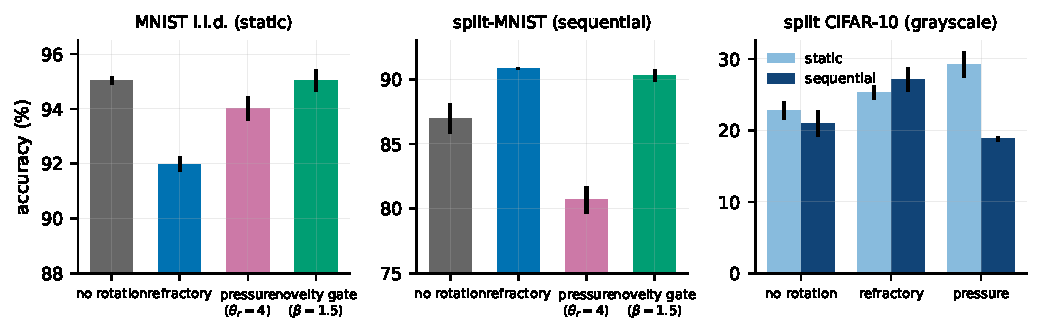
\includegraphics[width=\linewidth]{figs/fig_rotation.pdf}
\caption{\textbf{Rotation: price, trade-off, and gate.} Left: on i.i.d.\ MNIST the novelty gate
restores no-rotation accuracy. Middle: on split-MNIST rotation is required and the gate keeps it.
Right: on split CIFAR-10 (grayscale) rotation is a gain on \emph{both} axes.}
\label{fig:rotation}
\end{figure}

\section{Small buffers: what the night still buys}
\label{app:k200}

At $K{=}200$ the night appeared to keep a $\sim$2.6-point edge in our earlier phases; the final
triangulation (Figure~\ref{fig:k200}) dissolves most of it into a substrate mismatch. On the
\emph{same} $512$--$256$/$5\%$ substrate, the night reaches $84.0\pm3.4$ while noisy
pressure-burst local sleep reaches $84.3\pm1.0$ and local$+$night $84.8\pm0.9$ --- parity, with
three-fold smaller variance for the wake-side scheme. The strongest tiny-buffer number remains
the narrower $256$--$128$/$10\%$ night ($86.9$), so the offline window retains an advantage only
in combination with narrow substrates. The mechanism results stand: replay diversity (noise
$\sigma{=}0.2$) is specifically a wake-side lever --- it lifts every local scheme
($81.8\pm2.9\to84.3\pm1.0$) and \emph{hurts} the night ($84.0\to81.8\pm3.2$) --- and
\emph{unmasked}, rotation-free waking replay collapses ($71.0\pm1.7$): isolated rotating
replay beats it at every buffer size we tested.

\begin{figure}[t]
\centering
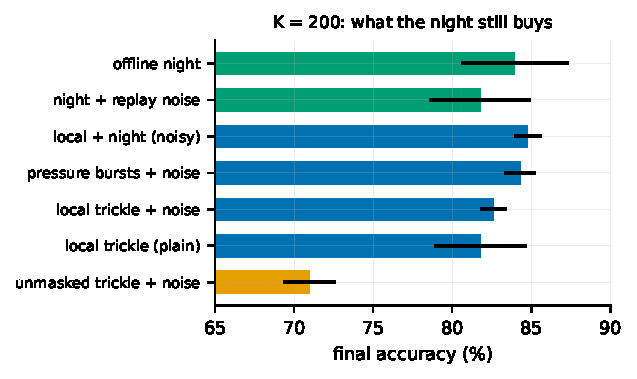
\includegraphics[width=.6\linewidth]{figs/fig_k200.pdf}
\caption{\textbf{$K=200$ mechanism triangulation.} Isolated rotating replay beats the unmasked trickle, diversity helps only during wake, and the irreducible advantage of the night at tiny buffers is its interference-free window.}
\label{fig:k200}
\end{figure}

\section{Sleep-anchored down-selection}
\label{app:downsel}

Motivated by the synaptic homeostasis hypothesis \citep{tononi2014}, we anchored structural
plasticity (prune the weakest fraction of live synapses, regrow the same number with a distance
bias) to consolidation windows, using the Kolen--Pollack decay of \eqref{eq:kp} as the natural
weakening force on unreplayed synapses. The verdict splits three ways at matched turnover
($\approx5\%$ per epoch). On the \emph{continuous} local-sleep substrate pruning is free
(sleep-anchored $90.9\pm0.2$, clocked $90.6\pm0.4$, none $90.8\pm0.1$). On the pure
\emph{night} substrate, pruning immediately after each night helps substantially
($87.2\pm3.8$ vs.\ $84.1\pm1.3$) --- offline down-selection rescues the wide-sparse night.
On the \emph{episodic-burst} substrate pruning is harmful ($84.6\pm0.5$ burst-anchored,
$86.6\pm1.3$ clocked, vs.\ $89.9\pm0.1$ without): when replay is rare, synapses are cut before
enough consolidation events have protected them. Down-selection, like replay itself, needs
either density or an offline window.


\section{Learning-rate sensitivity}
\label{app:eta}

The optimiser comparison invites an objection: SGD's $\eta$ was chosen, Adam's was left at its
default. A two-sided sweep dissolves it. At the $10\%$ record fraction (three seeds), heavy-ball
SGD under always-on rotation holds $92.2\pm0.7/93.3\pm0.2$ at $\eta{=}0.01$,
$92.7\pm0.3/94.7\pm0.3$ at $0.02$ (the joint optimum) and $91.5\pm0.6/94.7\pm0.3$ at $0.05$,
decaying at $0.005$ ($91.3/91.3$) and destabilising at $0.1$ ($79.5\pm17.3$), while masked
Adam has its optimum at the default ($91.8\pm0.6/94.6\pm0.2$ at $10^{-3}$; $89.9/89.9$ at
$3{\cdot}10^{-4}$, $90.9/94.3$ at $3{\cdot}10^{-3}$): the comparison of
Table~\ref{tab:ablation} is at each optimiser's best rate. The original sweep, at the $5\%$
fraction of the earlier phases, told the same story. There, under always-on rotation, SGD holds a sequential
plateau over $\eta\in[0.01,0.02]$ ($91.9\pm0.5$/$92.0\pm0.6$) and a static plateau over
$[0.02,0.05]$ ($93.3$--$93.7$), decaying gracefully outside ($86.3$/$89.2$ at $\eta{=}0.1$);
$\eta{=}0.02$ is the joint optimum. Masked Adam, swept over a tenfold range, has its
sequential optimum exactly at the default ($90.8\pm0.1$ at $10^{-3}$; $88.6$ at
$3{\cdot}10^{-4}$, $88.9$ at $3{\cdot}10^{-3}$) --- the comparison of
Section~\ref{sec:direction} was already at Adam's best --- and no Adam setting reaches the
heavy-ball joint point ($3{\cdot}10^{-3}$ buys $93.6$ static at a three-point sequential cost).
Unmasked SGD is poor and unstable at \emph{every} rate ($84$--$88$, seed deviations
$1.8$--$4.1$, three- to eight-fold those of the masked runs), making the stabilising role of isolation plus rotation (the unmasked runs are rotation-free) a
cross-$\eta$ fact. The bout-committed gate inherits the plateau, and the optimum
shifts one notch down on CIFAR ($\eta{=}0.01$).


\section{Probes of the residual static price}
\label{app:probes}

\paragraph{Single-pass streams.} With one epoch per task instead of five (everything else
as in the headline cells, three seeds), refractory local sleep reaches $91.8\pm0.2$ ($F{=}5.7$) against $91.6$ with five epochs,
BP+ER $88.7\pm0.3$, the offline night $75.1\pm3.5$ (one night per task is too few),
unmasked interleaved replay $76.0\pm20.1$ and no buffer $18.1$ (held-out split): the proposed system keeps its lead over every tested control in a
single pass, while the offline night falls below BP+ER.

\paragraph{Bout length and the OFF-side refractory.}
Bout length is a proper knob: $M{=}512$ (duties
$0.61/0.38$) gives $91.7\pm0.4/94.0\pm0.5$, already recovering most of what the per-batch gate
loses, while $M{=}4096$ drives the static duty to $0.94$ and the refund vanishes
($93.4\pm0.1$). The static ceiling of silent isolation ($96.0$) stays out of reach ---
rotation, even in bouts, keeps a residual price --- so the committed gate buys
regime-adaptivity, not a free lunch. Completing the flip-flop with an OFF-side refractory
(once a bout expires, triggers are ignored for $M_{\mathrm{off}}$ batches) is a clean null:
short refractories ($M_{\mathrm{off}}{\le}1024$) never engage on the static stream --- a bout
expires only after its trigger has been quiet for $M$ batches, so static re-triggering is not
flicker to begin with --- while a long one ($M_{\mathrm{off}}{=}4096$) lowers the static duty
to $0.53$ without moving static accuracy ($94.0\pm0.7$) and monotonically erodes the
sequential axis ($92.1\to91.0$, occasionally masking a task switch). Together with the
$M{=}512$ cell (duty $0.38$, static $94.0$), this locates the residual static price in the
rotation of settled coalitions itself, not in how often the gate fires.

\paragraph{Structural exemption and synaptic anchoring.}
\emph{Utility-exempt rotation} spares the top-$q$ units by long-term use trace from ever
being benched, so the settled coalitions stay awake. It traces a smooth trade-off between
always-on rotation and the rotation-free system ($q{=}0.10$: $90.9\pm0.1/94.2\pm0.2$;
$q{=}0.25$: $89.1\pm0.4/95.4\pm0.2$), but the bout gate beats the $q{=}0.10$ point by $+1.1$
sequential at equal static: \emph{temporal commitment dominates structural exemption},
recapitulating at the utility level what unit-level pressure gating showed earlier
(Figure~\ref{fig:rotation}) --- any structural narrowing of the rotation pool is paid for in
replay-channel width.

\emph{Two-timescale synapses} give every weight a slow anchor in the spirit of synaptic
consolidation cascades \citep{benna2016}: the fast weight decays toward its anchor at rate
$\lambda$ while the anchor absorbs it at rate $\mu$, ticking only on waking updates so the
exactness of the replay path is untouched. The strong hypothesis --- that settled function
living in the anchor would dissolve rotation's static price --- is falsified: across
$\lambda\in[3{\cdot}10^{-4},3{\cdot}10^{-3}]$, $\mu\in[10^{-4},10^{-3}]$ no cell exceeds
the anchor-free static accuracy, and strong coupling hurts both axes (the anchor becomes a
lagging drag). Weak symmetric coupling ($\lambda{=}\mu{=}3{\cdot}10^{-4}$), however, acts as
a \emph{sequential stabiliser}: $92.4\pm0.2$, the best sequential cell of the $5\%$ grid
with the seed variance halved, at static parity --- weakly dominating the $5\%$ always-on
point. Anchor and bout gate compose sub-additively
($92.3\pm0.3/93.8\pm0.5$, between the parents).


% ---------------------------------------------------------------- refs


\section{Isolation across replay batch sizes}
\label{app:isomargin}
Figure~\ref{fig:isomargin} extends the left panel of Figure~\ref{fig:batch} to two-sample
replay micro-batches and shows, per batch size, the seed-paired margin of the full system over
rotation with unmasked replay (held-out split; six seeds at batches $2$, $4$ and $16$, three at
$8$). From $16$ down to $4$ the margin is $0.1$ $[-0.3,+0.5]$, $0.3$ $[-0.2,+0.6]$ and $0.3$
$[-0.5,+1.2]$: isolation costs nothing and buys nothing measurable in mean accuracy while the
rotation keeps the live coalition tolerant of unmasked replay. At batch $2$ the replay
gradient is too noisy for either system --- the isolated one falls to $79.0\pm3.2$
(forgetting $21.5\pm4.2$ against $6.4$ at batch $16$), every seed between $75.5$ and $84.3$
--- but the unmasked one bifurcates: three seeds finish at $82.5$--$84.8$, slightly
\emph{above} their isolated counterparts ($+0.3$, $+1.8$, $+8.1$), one at $58.2$ and two at
chance ($9.9$). Leaking replay onto the live coalition is therefore not a pure loss --- the
surviving seeds show that the extra plasticity can help --- but it opens a failure mode that
the mask closes: with the current input's hidden computation held invariant, the noisiest
replay degrades the system gracefully instead of destroying it. The paired mean at batch $2$
($+24$ $[-0.2,+48.5]$) describes that failure mode, not a margin, and is kept out of the
ranges quoted in the main text.

\begin{figure}[h]
\centering
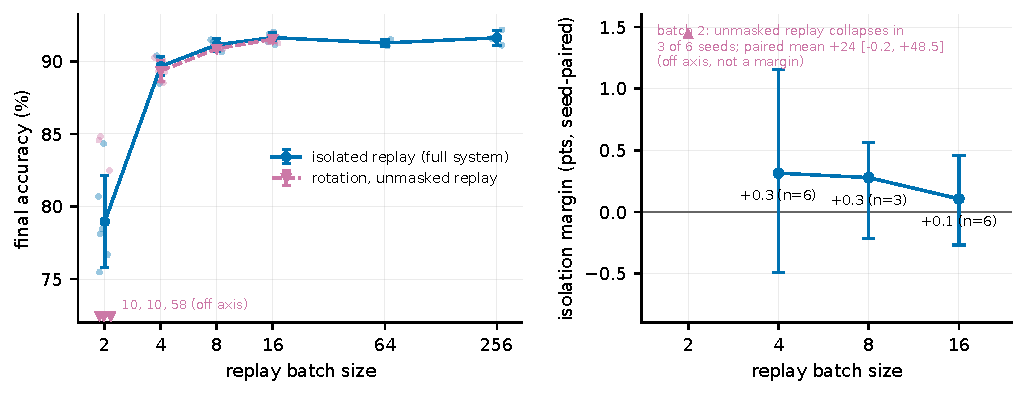
\includegraphics[width=.95\linewidth]{figs/fig_isomargin.pdf}
\caption{\textbf{Isolation across replay batch sizes} (held-out split). \textbf{Left:}
split-MNIST accuracy against replay batch size for isolated replay (the full system) and for
rotation with unmasked replay, every seed shown; at batch $2$ no unmasked mean is drawn
because three of six seeds fail (values at the axis floor). \textbf{Right:} the seed-paired
margin of isolation with a 95\% bootstrap interval at the batch sizes where the unmasked
run does not collapse.}
\label{fig:isomargin}
\end{figure}

\section{Development-phase numbers and a second held-out split}
\label{app:val}

Every configuration choice made during this project --- some four hundred sequential-axis
configurations over twenty phases --- was made on the official test sets, which served as
the development set; the paper reports numbers measured on a stratified tenth of the training
data held out from training and never used for any decision, with the remaining nine tenths
as the stream. Table~\ref{tab:val} places the development-phase numbers beside the reported
ones and beside a second, independent held-out tenth (a different split seed) for the
headline rows. Over the $87$ sequential configurations run under both protocols, reported
numbers sit $1.1$ points below the development numbers on average (a smaller training set
and a distribution-matched evaluation set both contribute) and rank-correlate with them at
Spearman $\rho=0.97$; every ordering carried by the paper holds on both held-out splits, with
one magnitude that does not: the same-substrate night, bimodal on the first split
($89.0\pm3.5$), reaches $91.5\pm0.5$ on the second and trails the full system by $0.3$ there.
The adaptive decay's static margin on MNIST is likewise split-dependent ($93.5\pm4.3$ with one
collapsed seed on the first split, $95.2\pm0.4$ on the second). Table~\ref{tab:accmatrix}
gives the per-task accuracy matrix of the headline configuration on the reported split.

\begin{table}[H]
\centering\small
\caption{\textbf{Development-phase (official test set) numbers beside the reported held-out
numbers and a second held-out split.} Sequential accuracy, with the static axis on its own row
where the paper reports it; six seeds on the reported split for the headline rows, three
elsewhere. Lower block: raw split CIFAR-10.}
\label{tab:val}
\begin{tabular}{@{}lccc@{}}
\toprule
& development (test) & reported (held-out) & second split \\
\midrule
always-on rotation (default) & $92.7\pm0.3$ & $91.6\pm0.3$ & $91.8\pm0.4$ \\
\quad static & $94.7\pm0.3$ & $94.1\pm0.2$ & $94.1\pm0.6$ \\
bout-committed gate & $92.3\pm0.2$ & $91.8\pm0.3$ & $92.0\pm0.6$ \\
rotation alone (unmasked replay) & $92.1\pm0.5$ & $91.5\pm0.3$ & $91.8\pm0.6$ \\
\quad static & $94.7\pm0.1$ & $93.7\pm0.3$ & $93.7\pm0.3$ \\
silent mask (no rotation) & $88.8\pm0.8$ & $88.0\pm0.7$ & $88.6\pm1.3$ \\
unmasked interleaved ER (SGD) & $87.0\pm1.1$ & $85.4\pm3.5$ & $80.0\pm14.1$ \\
BP $+$ ER & $89.3\pm0.8$ & $88.8\pm0.3$ & $88.5\pm0.7$ \\
offline night, same substrate & $90.9\pm3.2$ & $89.0\pm3.5$ & $91.5\pm0.5$ \\
offline night, narrow substrate & $90.7\pm0.4$ & $89.2\pm1.7$ & $89.3\pm0.6$ \\
adaptive $\lambda$ (drive) & $91.7\pm0.2$ & $90.6\pm0.6$ & $90.8\pm0.1$ \\
\quad static & $96.1\pm0.2$ & $93.5\pm4.3$ & $95.2\pm0.4$ \\
five hidden layers $+$ skips $+$ adaptive $\lambda$ & $91.5\pm0.4$ & $91.0\pm0.3$ & $91.1\pm0.3$ \\
\quad static & $96.2\pm0.3$ & $95.8\pm0.3$ & $95.7\pm0.1$ \\
no buffer & $19.6\pm0.0$ & $19.4\pm0.0$ & $19.5\pm0.0$ \\
\midrule
\multicolumn{4}{@{}l}{\emph{split CIFAR-10 (raw)}} \\
\quad rotation & $29.5\pm0.8$ & $28.9\pm1.0$ & $29.7\pm0.9$ \\
\quad offline night & $26.2\pm0.6$ & $25.7\pm1.2$ & $26.5\pm0.4$ \\
\quad BP $+$ ER & $25.1\pm1.5$ & $24.8\pm0.3$ & $25.8\pm0.8$ \\
\quad unmasked ER & $17.0\pm6.1$ & $15.4\pm4.2$ & $15.5\pm4.5$ \\
\quad no buffer & $16.4\pm0.2$ & $16.3\pm0.1$ & $16.6\pm0.0$ \\
\bottomrule
\end{tabular}
\end{table}

\begin{table}[H]
\centering\small
\caption{\textbf{Per-task accuracy matrix} of the headline configuration on split-MNIST
(held-out split, mean over six seeds): row $=$ after training task $i$, column $=$ accuracy on
task $j$. Forgetting $F$, the mean of the diagonal minus the last row over tasks $1$--$4$, is
$6.4\pm0.6$; the drop is concentrated on tasks $2$--$3$ and the first task is retained.}
\label{tab:accmatrix}
\begin{tabular}{lccccc}
\toprule
after task & T1 & T2 & T3 & T4 & T5 \\
\midrule
1 & $99.8$ & & & & \\
2 & $98.7$ & $97.2$ & & & \\
3 & $97.7$ & $92.7$ & $97.0$ & & \\
4 & $97.5$ & $89.6$ & $92.9$ & $97.5$ & \\
5 & $96.7$ & $88.1$ & $89.7$ & $91.5$ & $91.8$ \\
\bottomrule
\end{tabular}
\end{table}

\end{document}
